\documentclass[10pt]{article}
\usepackage{/Users/zhaor/MASTER/UNIVERSITY/NotesTeX/NotesTeX} %/Path/to/package should be replaced with package location
\usepackage{esvect}
\usepackage{cancel}
\graphicspath{ {./figures/} }

\title{{\Huge ECE286 - Probability and Statistics}\\{\Large{What is the probability of me passing this course}}}
\author{Regis Zhao\footnote{\href{https://google.com/}{\textit{TeX file on GitHub}}}}

\affiliation{University of Toronto}
\emailAdd{regis.zhao@mail.utoronto.ca}

\begin{document}

\maketitle
\flushbottom
\newpage

\pagestyle{fancynotes}

\part{Probability}

\section{Introduction}
\begin{itemize}
    \item probability comes from:
        \begin{itemize}
            \item things we can't model well
            \item good models but limited measurements
        \end{itemize}
    \item uncertainty is unavoidable, but probability helps describe uncertainty
\end{itemize}

\section{Sample Space}
\begin{definition}
    \textbf{Sample Space}: the set of all possible outcomes, $S$ 
    \begin{itemize}
        \item e.g. for 1 coin flip: $S = {H, T}$
    \end{itemize}
\end{definition}
\begin{itemize}
    \item each outcome in a sample space is called an \textbf{element} or \textbf{member}
\end{itemize}

\section{Events}
\begin{definition}
    \textbf{Event}: a subset of sample space $S$
     \begin{itemize}
        \item e.g. for a die: each element \{1, 2, 3, \ldots \} is an event, rolling even or rolling odd are events 
    \end{itemize}
\end{definition}
\begin{definition}
    The \textbf{complement} of an event $A$ with respect to $S$ : everything in $S$ that isn't in $A$ 
    \begin{itemize}
        \item denoted by $A'$
        \item e.g. for a die: \{1, 2\} is a complement of \{3, 4, 5, 6\}
    \end{itemize}
\end{definition}
\begin{definition}
    The \textbf{intersection} of two events $A$ and $B$ : everything in $A$ \textit{and} $B$
    \begin{itemize}
        \item denoted by $A \cap B$
        \item $A$ and $B$ are mutually exclusive if $A \cap B = \emptyset$ (empty set)
    \end{itemize}
\end{definition}
\begin{definition}
    The \textbf{union} of two events $A$ and $B$ : everything in $A$ or $B$ 
    \begin{itemize}
        \item denoted by $A \cup B$
        \item $A \cup A' = S$
    \end{itemize}
\end{definition}


\section{Counting}
\begin{theorem}
    \textbf{Generalized Multiplication Rule}: if an operation can be performed in $n_1$ ways, and if for each of these a second operation can be performed in $n_2$ ways, and for each of these \ldots, then the sequence of $k$ operations can be performed in $ n_1n_2\ldots n_k$ ways
\end{theorem}
\begin{itemize}
    \item e.g. Menu options: 3 appetizers, 4 mains, 2 deserts
    \item then there are $3 \cdot 4 \cdot 2 = 24$ options
\end{itemize}

\begin{definition}
    \textbf{Permutation}: an arrangement of all or part of a set of objects
\end{definition}
\begin{itemize}
    \item we can derive formula for permutations using the multiplication rule:
    \item for example: permutations of three letters a, b, and c
    \item there are 3 choices for first position, and no matter what you choose, there will be 2 choices for the second, and 1 choice for the third
    \item therefore: $(3)(2)(1) = 6$ permutations
\end{itemize}
\begin{theorem}
    The number of permutations of $n$ objects is $n!$.    
\end{theorem}
\begin{theorem}
    The number of permutations of $r$ out of $n$ items is
    \begin{align*}
        _nP_r = \frac{n!}{(n-r)!}
    .\end{align*}
\end{theorem}
\begin{theorem}
    The number of permutations of $n$ objects arranged in a circle is $(n-1)!$.
\end{theorem}

\subsection{Permutations with Identical Items}
\begin{theorem}
    Given $m$ kinds of items, and each kind of item has $n_k$ of them ($k = 1, 2, \ldots, m$), then the number of \textit{distinct} permuations is
    \begin{align*}
        {n \choose n_1, n_2, \ldots, n_m} = \frac{n!}{n_1! n_2! \ldots n_m!}
    .\end{align*}
\end{theorem}

\subsection{Partitions}
\begin{itemize}
    \item partitions divide a set into subsets
    \item often we want to find the number of possible ways to split a set up into partitions, where in each partition, the order doesn't matter
\end{itemize}
\begin{theorem}
    Given $m$ partitions of size $n_1, n_2, \ldots, n_m$, the number of ways of partitioning the set is 
    \begin{align*}
        {n \choose n_1, n_2, \ldots, n_m} = \frac{n!}{n_1! n_2! \ldots n_m!}
    .\end{align*}
\end{theorem}
\begin{itemize}
    \item note that this is the same formula as the number of permutations with identical items
    \item this is because once we put a group of items in a partition, their order doesn't matter anymore and they are essentially identical elements to us
\end{itemize}


\subsection{Combinations}
\begin{itemize}
    \item \textbf{combinations} are ways of selecting objects without regard to order
    \item combinations are like permutations except you don't care about order
    \item you can think of a size $r$ combination as paritioning a set into 2 cells, where one cell has size $r$ and the other is the rest of the set
        \begin{itemize}
            \item how many ways can you put items from a set into a size $r$ partition
        \end{itemize}
    \item using the partition formula:
\end{itemize}
\begin{theorem}
    The number of size $r$ combinations of $n$ distinct objects is
    \begin{align*}
        {n \choose r, n-r} = \frac{n!}{r!(n-r)!}
    ,\end{align*}
    or more commonly written as "$n$ choose $r$":
    \begin{align*}
        {n \choose r}
    .\end{align*}
\end{theorem}


\section{Probability of an Event}
\begin{itemize}
    \item a measure of the likelihood of an event happening -- a value ranging from 0 to 1
\end{itemize}
\begin{definition}
    The \textbf{probability} of an event $A$ in sample space $S$ is the sum of the weights of all sample points in $A$.
    \begin{align*}
        0 \le P(A) \le 1, \quad P(\emptyset) = 0, \quad \text{and} \quad P(S) = 1
    .\end{align*}
    \begin{itemize}
        \item if $A_1, A_2, A_3, \ldots$ is a sequence of mutually exclusive events, then
            \begin{align*}
                P(A_1 \cup A_2 \cup A_3 \cup \ldots) = P(A_1) + P(A_2) + P(A_3) + \ldots
            .\end{align*}
    \end{itemize}
\end{definition}

\subsection{Additive Rules}
\begin{theorem}
    \textbf{Additive Rule} (applies to unions of events): if $A$ and $B$ are two events, then
    \begin{align*}
        P(A \cup B) = P(A) + P(B) - P(A \cap B)
    .\end{align*}
    \begin{itemize}
        \item if $A$ and $B$ are mutually exclusive, then $A \cap B = \emptyset$ and
             \begin{align*}
                P(A \cup B) = P(A) + P(B)
            .\end{align*}
        \item if $A$ and $A'$ are complementary events, then
            \begin{align*}
                P(A) + P(A') = 1
            .\end{align*}
    \end{itemize}
\end{theorem}
\begin{figure}[h]
    \centering
    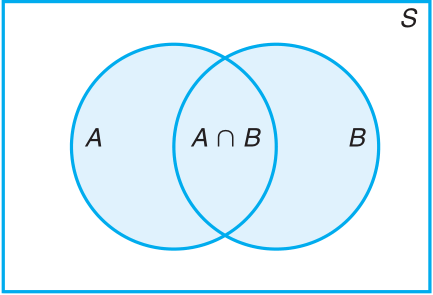
\includegraphics[width=0.4\textwidth]{additiveRule}
    \caption{Additive rule of probability}
    \label{fig:additiveRule}
\end{figure}
\begin{theorem}
    For three events $A$, $B$, and $C$,
    \begin{align*}
        P(A \cup B \cup C) &= P(A) + P(B) + P(C) \\ &- P(A \cap B) - P(A \cap C) - P(B \cap C) + P(A \cap B \cap C)
    .\end{align*}
\end{theorem}




\section{Conditional Probability, Independence, and the Product Rule}

\subsection{Conditional Probability}
\begin{itemize}
    \item \textbf{conditional probability} is the probability of an event $B$ occurring when it is known that some event $A$ has occurred
\end{itemize}
\begin{definition}
    The \textbf{conditional probability} of $B$, given $A$, is denoted by $P(B|A)$ and is defined by
    \begin{align*}
        P(B|A) = \frac{P(A \cap B)}{P(A)}, \quad \text{provided} \quad P(A) > 0
    .\end{align*}
\end{definition}
\begin{itemize}
    \item the probability of $B$ happening, given $A$, is equal to the probability of their intersection divided by the probability of $A$ happening
\end{itemize}

\subsection{Independence}
\begin{definition}
    $A$ and $B$ are independent if and only if 
        \begin{align*}
            P(A|B) = P(A) \quad \text{or} \quad P(B|A) = P(B)
        .\end{align*}
        \begin{itemize}
            \item probability of $A$ or $B$ happening doesn't depend on if the other event happened
            \item otherwise, $A$ and $B$ are \textbf{dependent}
        \end{itemize}
\end{definition}
\begin{itemize}
    \item the condition $P(B|A) = P(B)$ implies that $P(A|B) = P(A)$
    \item note that independence $\neq$ mutually exclusive
        \begin{itemize}
            \item e.g. head and tails are mutually exclusive but not independent ($P(H|T) = 0$)
        \end{itemize}
\end{itemize}

\subsection{Product Rule}
\begin{itemize}
    \item allows us to calculate the probability that two events will both occur
\end{itemize}
\begin{theorem}
    \textbf{Product Rule}: If in an experiment the events $A$ and $B$ can both occur, then
    \begin{align*}
        P(A \cap B) = P(A)P(B|A), \quad \text{provided} \quad P(A) > 0
    .\end{align*}
\end{theorem}
\begin{theorem}
    Two events $A$ and $B$ are independent if and only if
    \begin{align*}
        P(A \cap B) = P(A)P(B)
    .\end{align*}
    \begin{itemize}
        \item the probability that two independent events will both occur is equal to the product of their individual probabilities
        \item notice how this is a special case of the product rule $P(A \cap B) = P(A)P(B|A)$ where $P(B|A) = P(B)$ since $A$ and $B$ are independent
    \end{itemize}
\end{theorem}
\begin{theorem}
    \textbf{Product Rule for two or more events}: if the events $ A_1$, $ A_2$, \ldots, $A_k$ can occur, then
    \begin{align*}
        \text{refer to the textbook theorem 2.12 lol}
    .\end{align*}
    If the events $ A_1$, $ A_2$, \ldots, $A_k$ are independent, then
    \begin{align*}
        P(A_1 \cap A_2 \cap \ldots \cap A_k) = P(A_1)P(A_2)\ldots P(A_k)
    .\end{align*}
\end{theorem}



\section{Bayes' Rule}
\subsection{Total Probability}
\begin{itemize}
    \item addresses the problem of finding the total probability of something happening, when you know its conditional probabilities
    \item for example, what is the probability of a product being defective if it was produced by machines that each have a probability of creating defective products
\end{itemize}
\begin{theorem}
    If the events $ B_1$, $B_2$, \ldots, $B_k$ constitute a partition of the sample space $S$ such that $P(B_i) \neq 0$ for $i = 1, 2, \ldots k$, then for any event $A$ of $S$,
    \begin{align*}
        P(A) = \sum_{i=1}^{k} P(B_i \cap A) = \sum_{i=1}^{k} P(B_i)P(A|B_i)
    .\end{align*}
\end{theorem}
\begin{figure}[h]
    \centering
    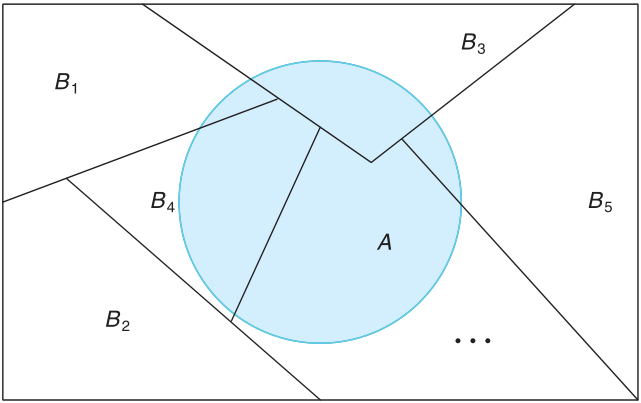
\includegraphics[width=0.5\textwidth]{totalProbability}
    \caption{Partitioning the sample space $S$. The probability of $A$ is the sum of the probabilities of the intersections between the partitions and $A$.}
    \label{fig:totalProbability}
\end{figure}

\subsection{Bayes' Rule}
\begin{itemize}
    \item addresses the problem of finding conditional probability, $P(B_i|A)$
    \item for example, what is the probability that a product was created by a certain machine, given that the product is defective
    \item recall formula for conditional probability, and substitute in the formula for total probability in the denominator:
\end{itemize}
\begin{theorem}
    \textbf{Bayes' Rule}: If the events $B_1$, $B_2$, \ldots, $B_k$ constitute a partition of the sample space $S$ such that $P(B_i) \neq 0$ for $i = 1, 2, \ldots, k$, then for any event $A$ in $S$ such that $P(A) \neq 0$, then the probability of a cell $B_n$ in the partition, given $A$, is given by 
    \begin{align*}
        P(B_n|A) = \frac{P(B_n \cap A)}{\sum_{i=1}^{k} P(B_i \cap A)} = \frac{P(B_n)P(A|B_n)}{\sum_{i=1}^{k} P(B_i)P(A|B_i)}
    .\end{align*}
\end{theorem}
\begin{itemize}
    \item recall the product rule, rearranging it, we get:
        \begin{align*}
            P(B|A) = \frac{P(B \cap A)}{P(A)} \quad \text{and} \quad P(A|B) = \frac{P(A \cap B)}{P(B)}
        .\end{align*}
    \item noting that $P(B \cap A) = P(A \cap B)$ , we can rearrange and equate the above equations:
        \begin{gather*}
            P(B|A)P(A) = P(A|B)P(B) \\ 
            \text{or} \\ 
            \frac{P(B|A)}{P(B)} = \frac{P(A|B)}{P(A)}
        .\end{gather*}
\end{itemize}


\newpage

\part{Random Variables and Probability Distributions}

\section{Concept of a Random Variable}
\begin{definition}
    \textbf{Random variable} (RV): a function that maps each element in the sample space to a real number
    \begin{itemize}
        \item we use capital letters, say $X$, to denote a random variable and use its corresponding small letter, $x$, for one of its values it can take on
    \end{itemize}
\end{definition}
\begin{definition}
    \textbf{Discrete RV}: $X$ takes on a finite or countable number of values \\ 
    \textbf{Continuous RV}: $X$ takes on values in an interval of $\mathbb{R}$
\end{definition}

\section{Discrete Probability Distributions}
\begin{definition}
    The set of ordered pairs (x, f(x)) is a \textbf{probability function}, \textbf{probability mass function} (PMF), or \textbf{probability distribution} of the discrete RV $X$ if, for each possible outcome $x$,
    \begin{enumerate}
        \item $f(x) \ge 0$
        \item $\sum_{x} f(x) = 1$
        \item P(X = x) = f(x)
    \end{enumerate}
\end{definition}
\begin{definition}
    The \textbf{cumulative distribution function} (CDF) $F(x)$ of a discrete random variable $X$ with PMF $f(x)$ is the probability of $X$ being less than or equal to $x$ :
    \begin{align*}
        F(x) = P(X \le x) = \sum_{t\le x} f(t), \quad \text{for} - \infty < x < \infty
    .\end{align*}
\end{definition}

\section{Continuous Probability Distributions}
\begin{itemize}
    \item for a continuous random variable, the probability of it assuming a specific value \textit{exactly} is 0 since there are infinite values
    \item but the probability of $X$ assuming a value in an interval is nonzero
\end{itemize}
\begin{definition}
    The function $f(x)$ is a \textbf{probability density function} (PDF) for the continuous RV $X$, defined over the set of real numbers, if 
    \begin{enumerate}
        \item $f(x) \ge 0, \quad \text{ for all} \quad x \in \mathbb{R}$
        \item $\int_{-\infty}^{\infty} f(x) dx = 1 $
        \item $P(a<X<b) = \int_{a}^{b} f(x) dx $
    \end{enumerate}
\end{definition} 
\begin{definition}
    The \textbf{cumulative distribution function} $F(x)$ of a continuous random variable $X$ with PDF $f(x)$ is
    \begin{align*}
        F(x) = P(X \le x) = \int_{-\infty}^{x} f(t) dt, \quad \text{for} \quad -\infty < x < \infty
    .\end{align*}
\end{definition}

\section{Joint Probability Distributions}
\begin{itemize}
    \item previous section only focused on 1D sample spaces
    \item when dealing with the simultaneous occurrence of two RVs:
\end{itemize}
\begin{definition}
    The function $f(x, y)$ is a \textbf{joint probability distribution} or \textbf{joint PMF} of the discrete random variables $X$ and $Y$ if
    \begin{enumerate}
        \item $f(x, y) \ge 0$ for all $(x, y)$
        \item $\sum_{x} \sum_{y} f(x, y) = 1$
        \item $P(X = x, Y = y) = f(x, y)$
    \end{enumerate}
    For any region $A$ in the $xy$ plane, $P\left[ (X, Y) \in A \right] = \sum \sum_{A} f(x, y)$.
\end{definition}
\begin{definition}
    The function $f(x, y)$ is a \textbf{joint density function} of the continuous random variables $X$ and $Y$ if 
    \begin{enumerate}
        \item $f(x,y) \ge 0$, for all $(x,y)$
        \item $\int_{-\infty}^{\infty} \int_{-\infty}^{\infty} f(x,y) dx dy = 1 $
        \item $P \left[ (X,Y) \in A \right] = \int \int_{A} f(x,y) dx dy $, for any region $A$ in the $xy$ plane
    \end{enumerate}
\end{definition}

\subsection{Marginal Distributions}
\begin{itemize}
    \item what if we know the joint distribution of two RVs but only care about one (want to obtain the probability distribution of an individual RV)
    \item simply integrate/add along the variable to eliminate
\end{itemize}
\begin{definition}
    The \textbf{marginal distributions} of $X$ alone and of $Y$ alone are 
    \begin{itemize}
        \item for the discrete case:
            \begin{align*}
                g(x) = \sum_{y} f(x,y) \quad \text{and} \quad h(y) = \sum_{x} f(x,y)
            .\end{align*}
        \item for the continuous case:
            \begin{align*}
                g(x) = \int_{-\infty}^{\infty} f(x,y) dy \quad \text{and} \quad h(y) = \int_{-\infty}^{\infty} f(x,y) dx  
            .\end{align*}
    \end{itemize}
\end{definition}
\begin{itemize}
    \item idea: marginal distribution is just the 'weighted average' of $f(x,y)$ over all possibilities of $x$ or $y$
\end{itemize}

\subsection{Conditional Distributions}
\begin{itemize}
    \item recall conditional probability
    \item conditional distributions take very similar form
\end{itemize}
\begin{definition}
    Let $X$ and $Y$ be two RVs. The \textbf{conditional distribution} of RVs (discrete or continuous) is
    \begin{gather*}
        f(y|x) = \frac{f(x,y)}{g(x)} \\ 
        f(x|y) = \frac{f(x,y)}{h(y)}
    .\end{gather*}
\end{definition}
\begin{itemize}
    \item if we want to find the probability that $X$ falls between $a$ and $b$, given $Y = y$ :
        \begin{gather*}
            P(a<X<b | Y=y) = \sum_{a<x<b} f(x|y) \\ 
            P(a<X<b | Y=y) = \int_{a}^{b} f(x|y) dx
        .\end{gather*}
\end{itemize}

\subsection{Statistical Independence}
\begin{definition}
    Let $X$ and $Y$ be RVs with joint distribution $f(x,y)$ and marginal distributions $g(x)$ and $h(y)$. $X$ and $Y$ are \textbf{statistically independent} if and only if
    \begin{align*}
        f(x,y) = g(x)h(y)
    .\end{align*}
    for all $(x,y)$ within their range.
\end{definition}
\begin{itemize}
    \item same idea applies for joint probability distributions of more than 2 RVs -- their joint probability distributions are simply the product of the marginal distributions if the RVs are statistically independent
\end{itemize}



\part{Mathematical Expectation}

\section{Mean of a Random Variable}
\begin{itemize}
    \item essentially calculating what value of $x$ is most likely to occur based on the probability distribution $f(x)$
\end{itemize}
\begin{definition}
    Let $X$ be an RV with probability distribution $f(x)$. The \textbf{mean}, or \textbf{expected value} of $X$ is  
    \begin{itemize}
        \item for discrete case:
            \begin{align*}
                \mu = E(X) = \sum_{x} xf(x)
            .\end{align*}
        \item for continuous case:
            \begin{align*}
                \mu = E(X) = \int_{-\infty}^{\infty} xf(x) dx 
            .\end{align*}
    \end{itemize}
\end{definition}
\begin{itemize}
    \item notice: we mutliply the value of $x$ with its own probability so that values of $x$ with higher probability have a greater influence on what the expected value is
\end{itemize}
\begin{definition}
    Let $X$ be an RV with probability distribution $f(x)$. We define a new RV as a function of $X$, $g(X)$. The expectation of the RV $g(X)$ is 
    \begin{itemize}
        \item for discrete case:
            \begin{align*}
                \mu_{g(X)} = E [g(X)] = \sum_{x} g(x) f(x)
            .\end{align*}
        \item for continuous case:
            \begin{align*}
                \mu_{g(X)} = E[g(X)] = \int_{-\infty}^{\infty} g(x)f(x) dx 
            .\end{align*}
    \end{itemize}
\end{definition}
\begin{definition}
    Let $X$ and $Y$ be RVs with joint probability distribution $f(x,y)$. The expectation of the RV $g(X,Y)$ is 
    \begin{itemize}
        \item for discrete case:
            \begin{align*}
                \mu_{g(X,Y)} = E[g(X,Y)] = \sum_{x} \sum_{y} g(x,y)f(x,y)
            .\end{align*}
        \item for continuous case:
            \begin{align*}
                \mu_{g(X,Y)} = E[g(X,Y)] = \int_{-\infty}^{\infty} \int_{-\infty}^{\infty} g(x,y) f(x,y) dx dy  
            .\end{align*}
    \end{itemize}
\end{definition}
\begin{itemize}
    \item generalization of the calculation of mathematical expectations of functions of more than 2 RVs is straightforward
\end{itemize}


\section{Variance and Covariance of Random Variables}
\subsection{Variance}
\begin{itemize}
    \item measures how spread out a distribution is -- the variability of an RV
\end{itemize}
\begin{definition}
    Let $X$ be an RV with probability distribution $f(x)$ and mean $\mu = E(X)$. The \textbf{variance} of $X$ is
    \begin{itemize}
        \item if $X$ is discrete:
            \begin{align*}
                \sigma^2 = E[(X-\mu)^2] = \sum_{x} (x-\mu)^2 f(x)
            .\end{align*}
        \item if $X$ is continuous:
            \begin{align*}
                \sigma^2 = E[(X-\mu)^2] = \int_{-\infty}^{\infty} (x-\mu)^2 f(x) dx 
            .\end{align*}
    \end{itemize} 
    The positive square root of the variance, $\sigma$, is called the \textbf{standard deviation} of $X$.
\end{definition}
\begin{itemize}
    \item sometimes, variance is written as $var(X)$
    \item the $x-\mu$ centers the distribution on the y-axis
    \item squaring it allows for points at a greater distance from the mean $\mu$ to have a larger contribution, therefore measuring how spread out the distribution is
\end{itemize}
\begin{theorem}
    The variance of an RV $X$ is
    \begin{align*}
        \sigma^2 = E(X^2) - \mu^2
    .\end{align*}
    \begin{itemize}
        \item proof is in section 4.2 of textbook
    \end{itemize}
\end{theorem}

\subsection{Covariance}
\begin{itemize}
    \item measures the joint variability of two variables -- the direction of the relationship between two variables
        \begin{itemize}
            \item if large values of both variables occur together, covariance is positive
            \item if large values of one correspond to small values of the other RV, covariance is negative
        \end{itemize}
\end{itemize}
\begin{definition}
    Let $X$ and $Y$ be RVs with joint probability distribution $f(x,y)$. The \textbf{covariance} of $X$ and $Y$ is 
    \begin{itemize}
        \item if $X$ and $Y$ are discrete:
            \begin{align*}
                \sigma_{XY} = E[(X-\mu_X)(Y-\mu_Y)] = \sum_{x} \sum_{y} (x-\mu_X)(y-\mu_Y)f(x,y)
            .\end{align*}
        \item if $X$ and $Y$ are continuous:
            \begin{align*}
                \sigma_{XY} = E[(X-\mu_X)(Y-\mu_Y)] = \int_{-\infty}^{\infty} \int_{-\infty}^{\infty} (x-\mu_X)(y-\mu_Y)f(x,y) dx dy
            .\end{align*}
    \end{itemize}
\end{definition}
\begin{itemize}
    \item also written as $cov(X,Y)$
\end{itemize}
\begin{theorem}
    The covariance of two random variables $X$ and $Y$ with means $\mu_X$ and $\mu_Y$ is given by
    \begin{align*}
        \sigma_{XY} = E(XY) - \mu_X \mu_Y
    .\end{align*}
\end{theorem}

\subsection{Correlation Coefficient}
\begin{itemize}
    \item the sign of covariance provides information about the nature of the relationship between two variables, but the magnitude does not indicated anything about the \textit{strength} of the relationship since covariance isn't scale-free
        \begin{itemize}
            \item its magnitude depends on the units used to measure $X$ and $Y$
        \end{itemize}
    \item the scale-free version of covariance is called the correlation coefficient:
\end{itemize}
\begin{definition}
    Let $X$ and $Y$ be RVs with covariance $\sigma{XY}$ and standard deviations $\sigma_X$ and $\sigma_Y$. The \textbf{correlation coefficient} of $X$ and $Y$ is 
    \begin{align*}
        \rho_{XY} = \frac{\sigma_{XY}}{\sigma_X \sigma_Y}
    .\end{align*}
\end{definition}
\begin{itemize}
    \item like covariance, but normalized
    \item magnitude tells us \textit{strength} of relationship 
    \item $-1 \le \rho_{XY} \le 1$
    \item 'uncorrelated' if $\rho_{XY} = 0$
        \begin{itemize}
            \item since that would mean $\sigma_{XY} = 0$
        \end{itemize}
\end{itemize}


\section{Means and Variances of Linear Combinations of Random Variables}
\subsection{Means of LCs of RVs}
\begin{itemize}
    \item \textbf{expectation is linear} 
\end{itemize}
\begin{theorem}
    If $a$ and $b$ are constants, then
    \begin{align*}
        E(aX+b) = aE(X)+b
    .\end{align*}
\end{theorem}
\begin{theorem}
    The expectation of the sum or difference of two or more functions of an RV is the sum or difference of the expectations of the functions, i.e.
    \begin{align*}
        E[g(X) \pm h(X)] = E[g(X)] \pm E[h(X)]
    .\end{align*}
\end{theorem}

\subsection{Variances of LCs of RVs}
\begin{theorem}
    Let $X$ and $Y$ be two independent RVs. Then
    \begin{align*}
        E(XY) = E(X)E(Y)
    .\end{align*}
\end{theorem}
\begin{itemize}
    \item recall formula for covariance:
        \begin{align*}
            \sigma_{XY} = E(XY) - E(X)E(Y)
        .\end{align*}
    \item if $X$ and $Y$ are independent, then $E(XY) = E(X)E(Y)$, so:
\end{itemize}
\begin{theorem}
    Let $X$ and $Y$ be two independent RVs. Then $\sigma_{XY} = 0$
\end{theorem}
\begin{itemize}
    \item i.e. independence implies uncorrelated
    \item but uncorrelated does not imply independence
    \item independece is a stronger property than uncorrelated
\end{itemize}
\begin{theorem}
    The variance of $aX + bY + c$, where $a$, $b$, and $c$ are constants, is 
    \begin{align*}
        \sigma_{aX + bY + c}^2 = a^2\sigma_X^2 + b^2\sigma_Y^2 + 2ab\sigma_{XY}
    .\end{align*}
\end{theorem}
\begin{itemize}
    \item notice that $c$ has no effect on the variance -- the variance is unchanged if a constant is added or subtracted from an RV
         \begin{itemize}
            \item it simply shifts the values of the RV left or right, it doesn't change the variability
        \end{itemize}
    \item also notice that if $X$ and $Y$ are independent, then the last term is 0
    \item multiplying an RV by a constant scales the variance by the square of the constant, i.e. 
\end{itemize}
\begin{theorem}
    The variance of $aX$, where $a$ is a constant, is $\sigma^2_{aX} = a^2\sigma_X^2$
\end{theorem}



\newpage

\part{Common Discrete Probability Distributions}
\section{Uniform Distribution}
\begin{itemize}
    \item every element in $S$ has the same probability (e.g. coin flip)
    \item if $S = {1, 2, \ldots, n}$, then $f(k) = \frac{1}{n}$ for $k \in S$
\end{itemize}

\section{Binomial Distribution}
\begin{definition}
    \textbf{Binomial Distribution}: the probability of $x$ successes in $n$ trials for a binomial experiment:
    \begin{align*}
        b(x;n,p) = {n \choose x} p^x (1-p)^{n-x}
    .\end{align*}
\end{definition}
\begin{theorem}
    The mean and variance of the binomial distribution are 
    \begin{align*}
        \mu = np \quad \text{and} \quad \sigma^2 = np(1-p)
    .\end{align*}
\end{theorem}

\section{Multinomial Distribution}
\begin{itemize}
    \item like binomial but each trial has more than 2 possibilities, $E_1$, $E_2$, \ldots, $E_k$, where $k$ is the number of possibilities a trial can take on
\end{itemize}
\begin{definition}
    \textbf{Multinomial Distribution}: the probability of $E_1$ happening  $x_1$ times, $E_2$ happening $x_2$ times, \ldots, $E_k$ happening $x_k$ times, where $x_1 + x_2 + \ldots + x_k = n$:
    \begin{align*}
        f(x_1, x_2, \ldots, x_k; p_1, p_2, \ldots, p_k, n) = {n \choose x_1, x_2, \ldots, x_k} p_1^{x_1} p_2^{x_2} \ldots p_k^{x_k}
    .\end{align*}
\end{definition}

\section{Hypergeometric Distribution}
\begin{definition}
    \textbf{Hypergeometric Distribution}: given that there are a set amount of successes $K$ in a sample space of size $N$, what is the probability of selecting $x$ successes if you select $n$ times (with replacement)
    \begin{gather*}
        h(x;N,n,K) = \frac{{K \choose x} {N-K \choose n-x}}{{N \choose n}}, \quad \quad (n-x \le N-K)
    .\end{gather*}
    \begin{itemize}
        \item mean and variance:
            \begin{gather*}
                \mu = \frac{nK}{N} \quad \text{and} \quad \sigma^2 = \frac{N-n}{N-1}\cdot n\cdot \frac{K}{N}\left( 1-\frac{K}{N} \right) 
            .\end{gather*}
    \end{itemize}
\end{definition}

\section{Negative Binomial Distribution}
\begin{definition}
    \textbf{Negative Binomial Distribution}: probability of the $k$-th success occuring on the $x$-th trial, where the probability of a success is $p$
    \begin{gather*}
        b^*(x;k,p) = {x-1 \choose k-1} p^k(1-p)^{x-k}
    .\end{gather*}
    \begin{itemize}
        \item note:
            \begin{gather*}
                b^*(x;k,p) = pb(k-1;x-1,p)
            .\end{gather*}
    \end{itemize}
\end{definition}


\subsection{Geometric Distribution}
\begin{definition}
    \textbf{Geometric Distribution}: a special case of the negative binomial distribution, where $k=1$, i.e. probability of the first success happening on the $x^{th}$ trial
    \begin{gather*}
        g(x;p) = b^*(x;1,p) = p(1-p)^{x-1}
    .\end{gather*}
    \begin{itemize}
        \item mean and variance: 
            \begin{gather*}
                \mu = \frac{1}{p} \quad \text{and} \quad \sigma^2 = \frac{1-p}{p^2}
            .\end{gather*}
    \end{itemize}
\end{definition}

\section{Poisson Distribution}
\begin{itemize}
    \item like binomial except number of trials is continuous over some interval ($n \to \infty$)
    \item properties of a \textbf{Poisson Process}:
        \begin{enumerate}
            \item the number of outcomes in one time interval is independent of the number that occur in any other interval -- the Poisson process has no memory 
            \item the probability that a single outcome will occur during an interval is proportional to the length of the interval and doesn't depend on the number of outcomes occurring outside this interval
        \end{enumerate}
\end{itemize}
\begin{definition}
    \textbf{Poisson Distribution}: the probability distribution of a Poisson random variable $X$, representing the number of outcomes occurring in a given time interval or specified region denoted by $t$, is 
    \begin{gather*}
        p(x; \lambda t) = \frac{e^{-\lambda t}(\lambda t)^x}{x!}, \quad x = 0, 1, \ldots
    .\end{gather*}
    where $\lambda$ is the average number of outcomes per unit interval
    \begin{itemize}
        \item mean and variance are both given by 
            \begin{gather*}
                \mu = \sigma^2 = \lambda t
            .\end{gather*}
        \item note: the binomial distribution $b(x;n,p)$ becomes the Poisson distribution $p(x;\mu)$ as the sample size $n \to \infty$
    \end{itemize}
\end{definition}



\newpage
\part{Continuous Probability Distributions}
\section{Continuous Uniform Distribution}
\begin{definition}
    \textbf{Continuous Uniform Distribution}:
    \begin{gather*}
        f(x;A,B) = \begin{cases}
            \frac{1}{B-A}, & A \le x \le B \\ 
            0, & \text{elsewhere}
        \end{cases}
    .\end{gather*}
    \begin{itemize}
        \item the mean and variance are given by 
            \begin{gather*}
                \mu = \frac{A+B}{2} \quad \text{and} \quad \sigma^2 = \frac{(B-A)^2}{12}
            .\end{gather*}
    \end{itemize}
\end{definition}

\section{Normal Distribution}
\begin{itemize}
    \item the most important continuous probability distribution in the entire field of statistics 
    \item also known as the \textbf{Gaussian distribution} 
    \item a continuous random variable $X$ have the bell-shaped distribution of the normal curve is called a \textbf{normal random variable} 
\end{itemize}
\begin{definition}
    \textbf{Normal/Gaussian Distribution}:
    \begin{gather*}
        n(x;\mu,\sigma) = \frac{1}{\sqrt{2\pi}\sigma}e^{-\frac{1}{2\sigma^2}(x-\mu)^2}
    .\end{gather*}
    \begin{itemize}
        \item the mode occurs at the maximum, when $x=\mu$
        \item it is symmetric about  $x=\mu$
        \item points of inflection occur at $x=\mu \pm \sigma$
    \end{itemize}
\end{definition}

\subsection{Standard Normal Distribution}
\begin{itemize}
    \item calculating areas under the normal curve is important to obtain probabilities, but it's rather dumb to make tables of values for every single value of $\mu$ and $\sigma^2$
    \item instead, we are able to transform all observations of any normal RV $X$ into a new set of observations of a normal RV $Z$ with mean 0 and variance 1:
         \begin{gather*}
            Z = \frac{X-\mu}{\sigma}
        .\end{gather*}
\end{itemize}
\begin{definition}
    \textbf{Standard Normal Distribution}: special case of the normal distribution where $\mu=0$ and $\sigma^2 = 1$ 
\end{definition}

\section{Normal Approximation to the Binomial Distribution}
\begin{theorem}
    if $X$ is a binomial RV with $\mu = np$ and $\sigma^2 = np(1-p)$, then the limiting form of the distribution of
     \begin{gather*}
        Z = \frac{X-np}{\sqrt{np(1-p)}}
    .\end{gather*}
    as $n \to \infty$ is the standard normal distribution $n(z;0,1)$
\end{theorem}

\section{Gamma and Exponential Distributions}
\begin{itemize}
    \item the \textbf{Gamma function} is given by 
        \begin{gather*}
            \Gamma(\alpha)  = \int_{0}^{\infty} x^{\alpha-1}e^{-x} dx, \quad \quad \text{for} \; \alpha > 0
        .\end{gather*}
    \item properties of the Gamma function:
        \begin{enumerate}
            \item $\Gamma(n) = (n-1)(n-2)\ldots(1)\Gamma(1)$, for a positive integer $n$
            \item  $\Gamma(n) = (n-1)!$ for a positive integer $n$
            \item  $\Gamma(1) = 1$ 
            \item $\Gamma(\frac{1}{2}) = \sqrt{\pi} $
        \end{enumerate}
\end{itemize}
\begin{definition}
    \textbf{Gamma Distribution}:
    \begin{gather*}
        f(x;\alpha, \beta) = \begin{cases}
            \frac{1}{\beta^\alpha \Gamma(\alpha)}x^{\alpha-1}e^{-x / \beta}, & x>0 \\ 
            0, & \text{elsewhere}
        \end{cases}
    .\end{gather*}
    where $\alpha,\beta > 0$
    \begin{itemize}
        \item mean and variance: 
            \begin{gather*}
                \mu = \alpha \beta \quad \text{and} \quad \sigma^2 = \alpha \beta^2
            .\end{gather*}
    \end{itemize}
\end{definition}
\begin{definition}
    \textbf{Exponential Distribution}: special case of Gamma distributiion where $\alpha = 1$
     \begin{gather*}
        f(x;\beta) = \begin{cases}
            \frac{1}{\beta}e^{-x / \beta}, & x>0 \\ 
            0, & \text{elsewhere}
        \end{cases}
    .\end{gather*}
    where $\beta > 0$
    \begin{itemize}
        \item mean and variance: 
            \begin{gather*}
                \mu = \beta \quad \text{and} \quad \sigma^2 = \beta^2
            .\end{gather*}
    \end{itemize}
\end{definition}

\section{Chi-Squared Distribution}
\begin{definition}
    \textbf{Chi-Square Distribution}: special case of Gamma distribution where $\alpha = v / 2$, $\beta = 2$, and $v$ is a positive integer and is the only parameter, called the \textbf{degrees of freedom}
    \begin{gather*}
        f(x;v) = \begin{cases}
            \frac{1}{2^{v / 2}\Gamma(v / 2)}x^{v / 2 - 1} e^{-x / 2}, & x>0 \\ 
            0, & \text{elsewhere}
        \end{cases}
    .\end{gather*}
    \begin{itemize}
        \item mean and variance: 
            \begin{gather*}
                \mu = v \quad \text{and} \quad \sigma^2 = 2v
            .\end{gather*}
    \end{itemize}
\end{definition}

\section{Weibull Distribution}
\begin{definition}
    \textbf{Weibull Distribution}:
    \begin{gather*}
        f(x;\alpha, \beta) = \begin{cases}
            \alpha\beta x^{\beta-1}e^{-\alpha x^\beta}, &x>0 \\ 
            0, & \text{elsewhere}
        \end{cases}
    .\end{gather*}
    where $\alpha, \beta >0$
     \begin{itemize}
        \item its cumulative function is given by 
            \begin{gather*}
                F(x) = 1-e^{-\alpha x^\beta}
            .\end{gather*}
    \end{itemize}
\end{definition}





\newpage
\part{Functions of Random Variables}
\section{Transformations of Variables}
\begin{theorem}
    Suppose $X$ is a \textbf{discrete} RV with probability distribution $f(x)$. Let $Y = u(X)$ define a one-to-one transformation between values of $X$ and $Y$ so that we can also write $x = w(y)$. Then the probability distribution of $Y$ is
    \begin{align*}
        g(y) = f(w(y))
    .\end{align*}
    \begin{itemize}
        \item for the case of joint probability distributions $f(x_1, x_2)$, the probability distribution of $Y$ is 
            \begin{align*}
                g(y_1, y_2) = f[w_1(y_1, y_2), w_2(y_1, y_2)]
            .\end{align*}
    \end{itemize}
\end{theorem}
\begin{theorem}
    For the case where the RV is \textbf{continuous}, the probability distribution of $Y$ is 
    \begin{align*}
        g(y) = f(w(y))|J|
    .\end{align*}
    where $J = w'(y)$ is the \textbf{Jacobian} of the transformation.
    \begin{itemize}
        \item for joint probability distributions:
            \begin{align*}
                g(x_1, x_2) = f[w_1(y_1, y_2), w_2(y_1, y_2)]
            .\end{align*}
            where the Jacobian is the determinant of the Jacobian matrix

    \end{itemize}
\end{theorem}

\section{Moments and Moment-Generating Functions}
\begin{definition}
    The $r$ th \textbf{moment about the origin} of the RV $X$ is given by 
    \begin{gather*}
        \mu'_r = E(X^r) = \int_{-\infty}^{\infty} x^r f(x) dx 
    .\end{gather*}
\end{definition}
\begin{itemize}
    \item we can write mean and variance of a random variable in terms of moments: 
        \begin{gather*}
            \mu = \mu'_1 \quad \text{and} \quad \sigma^2 = \mu'_2 - \mu^2
        .\end{gather*}
\end{itemize}

\begin{definition}
    \textbf{Moment-generating function} of the RV $X $: alternative procedure for determining moments 
    \begin{gather*}
        M_X(t) = E(e^{tX}) = \int_{-\infty}^{\infty} e^{tx} f(x) dx 
    .\end{gather*}
\end{definition}
\begin{itemize}
    \item moment-generating functions will exist only if the integral in the above definition converges 
    \item if it exists, a moment-generating function of RV $X$ can be used to generate all the moments of that variable using the below method:
\end{itemize}
\begin{theorem}
    Let $X$ be a random variable with moment-generating function $M_X(t)$, then 
    \begin{gather*}
        \left. \frac{d^r M_X(t)}{d t^r} \right|_{t=0} = \mu'_r
    .\end{gather*}
\end{theorem}
\begin{theorem}
    \textbf{Uniqueness Theorem}: Let $X$ and $Y$ be two RVs with moment-generating functions $M_X(t)$ and $M_Y(t)$. If $M_X(t)=M_Y(t)$ for all values of $t$, then $X$ and $Y$ have the same probability distribution.
\end{theorem}
\begin{theorem}
    \begin{enumerate}
        \item $M_{X+a}(t) = e^{at}M_X(t)$ 
        \item $M_{aX}(t) = M_X(at)$
    \end{enumerate}
\end{theorem}
\begin{theorem}
    If $X_1, \ldots, X_n$ are independent RVs with moment-generating functions, and $Y = X_1 + \ldots + X_n$ then 
    \begin{gather*}
        M_Y(t) = M_{X_1}(t)M_{X_2}(t)\ldots M_{X_n}(t)
    .\end{gather*}
\end{theorem}

\subsection{Linear Combinations of Random Variables}
\begin{theorem}
    If $X_1, X_2, \ldots, X_n$ are independent RVs having normal distributions with means $\mu_1, \mu_2, \ldots, \mu_n$ and variances $\sigma_1^2, \sigma_2^2, \ldots, \sigma_n^2$, then the RV
    \begin{gather*}
        Y = a_1X_1 + a_2X_2 + \ldots + a_nX_n
    .\end{gather*}
    has a normal distribution with mean
    \begin{gather*}
        \mu_Y = a_1\mu_1 + a_2\mu_2 + \ldots + a_n\mu_n
    .\end{gather*}
    and variance 
    \begin{gather*}
        \sigma_Y^2 = a_1^2 \sigma_1^2 + a_2^2 \sigma_2^2 + \ldots + a_n^2 \sigma_n^2
    .\end{gather*}
\end{theorem}









\newpage

\part{Sampling}
Why sample?
\begin{itemize}
    \item can't measure entire population
    \item random sampling ensures sample reflects population
\end{itemize}

\section{Measures of Location: Sample Mean and Median}
\begin{itemize}
    \item Given sample data: $x_1, \ldots, x_n$
\end{itemize}
\begin{definition}
    \textbf{Sample Mean}: the numerical average
    \begin{align*}
        \overline{x} = \frac{1}{n} \sum_{i=1}^n x_i
    .\end{align*}
\end{definition}
\begin{definition}
    \textbf{Sample Median}: given that $ x_1, x_2, \ldots, x_n$ are arranged in increasing order of magnitude,
    \begin{align*}
        x_m =
        \begin{cases}
            x_{\frac{n+1}{2}} & \text{if $n$ odd} \\ 
            \frac{1}{2}\left( x_{\frac{n}{2}} + x_{\frac{n}{2}+1} \right) & \text{if $n$ even}
        \end{cases}
    .\end{align*}
    \begin{itemize}
        \item purpose of the sample median is to reflect the central tendency of the sample in a way that is uninfluenced by extreme values or outliers (unlike the mean)
    \end{itemize}
\end{definition}
\begin{definition}
    \textbf{Mode}: most frequently occurring value
    \begin{itemize}
        \item e.g. 1, 1, 1, 1, 1, 8
        \item mode = 1
    \end{itemize}
\end{definition}

\section{Measures of Variability}
\subsection{Sample Range and Sample Standard Deviation}
\begin{itemize}
    \item \textbf{sample range} is given by $X_{max} - X_{min}$
\end{itemize}
\begin{definition}
    \textbf{Sample Variance}, denoted by $s^2$, is given by
    \begin{align*}
        s^2 = \frac{1}{n-1} \sum_{i=1}^n \left( x_i - \overline{x} \right)^2
    .\end{align*}
    The \textbf{sample standard deviation}, denoted by $s$, is the positive square root of $s^2$:
    \begin{gather*}
        s = \sqrt{s^2}
    .\end{gather*}
\end{definition}
\begin{itemize}
    \item the quantity $n-1$ is often called the \textbf{degrees of freedom associated with the variance}
    \item this is because in general, $\sum_{i=1}^{n} (x_i-\overline{x}) = 0$, so the last value in the sample can be determined only using the first $n-1$ values
    \item this means the computation of sample variance doesn't involve all $n$ independent squared deviations from the mean
    \item there are only $n-1$ "pieces of information" that produce $s^2$ 
    \item therefore: there are $n-1$ degrees of freedom instead of $n$ when computing sample variance
\end{itemize}



\section{Visualization}
\subsection{Histogram}
\begin{itemize}
    \item plots the frequency of each outcome
    \item also can plot relative frequency:
    \item dividing each class frequency by the total number of observations, we obtain the relative frequency of each class interval
    \item we can plot relative frequency in a histogram
        \begin{figure}[H]
            \centering
            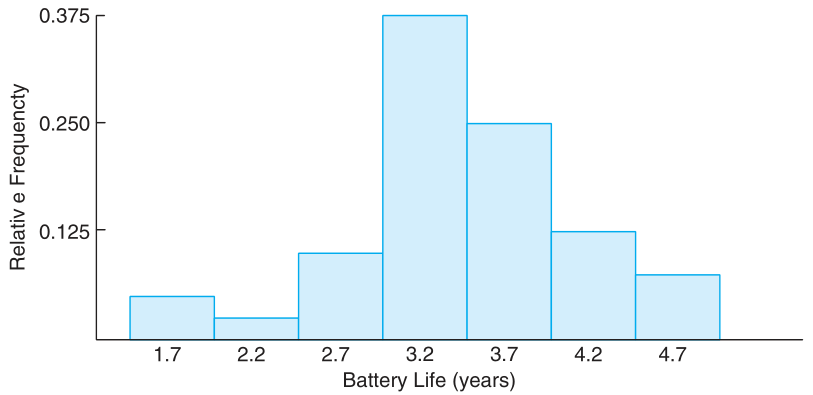
\includegraphics[width=0.8\textwidth]{histogram}
            \caption{Example of relative frequency histogram.}
            \label{fig:histogram}
        \end{figure}
\end{itemize}

\subsection{Box-and-Whisker Plot}
\begin{itemize}
    \item displays the center of location, variability, and degree of asymmetry
    \item encloses the \textit{interquartile range} of the data in a box which also displays the median within
    \begin{itemize}
        \item essentially encloses the middle 50\% of the data
    \end{itemize}
    \item the extremes of the interquartile range are the 75th percentile (upper quartile) and 25th percentile (lower quartile)
    \item "whiskers" extend from the sides of the box showing extreme observations
    \item outliers may be plotted as points as well
        \begin{figure}[H]
            \centering
            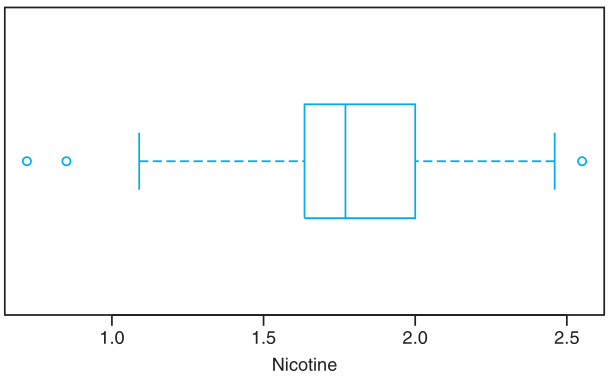
\includegraphics[width=0.8\textwidth]{boxAndWhisker}
            \caption{Example of box and whisker plot.}
            \label{fig:boxAndWhisker}
        \end{figure}
\end{itemize}






\part{Sampling Distributions}
\section{Random Sampling}
\begin{definition}
    A \textbf{population} consists of all possible observations.
\end{definition}
\begin{definition}
    A \textbf{sample} is a subset of a population.
    \begin{itemize}
        \item we work with samples because it is impractical to observe whole population
    \end{itemize}
\end{definition}
\begin{definition}
    Let $X_1, X_2, \ldots, X_n$ be $n$ independent random variables, each having the same probability distribution $f(x)$. Define $X_1, X_2, \ldots, X_n$ to be a \textbf{random sample} of size $n$ from the population $f(x)$ and write its joint probability as 
    \begin{gather*}
        f(x_1, x_2, \ldots x_n) = f(x_1)f(x_2)\ldots f(x_n)
    .\end{gather*}
\end{definition}

\section{Statistics and Sampling Distributions}
\begin{definition}
    \textbf{Statistic}: Any function of the random variables constituting a random sample (e.g. mean, median, variance, etc.).
\end{definition}
\begin{itemize}
    \item a sample is biased if it consistently over- or underestimates a statistic of interest
\end{itemize}

\begin{definition}
    \textbf{Sampling Distribution}: The probability distribution of a statistic.
\end{definition}
\begin{itemize}
    \item the sampling distribution of a statistic depends on the distribution of the population, size of samples, and method of choosing samples
    \item it is \textbf{very important to notice and understand (for pretty much the rest of the course) that the mean and variance of a \textit{statistic} is not the same as the mean and variance for the \textit{population}}
\end{itemize}

\section{Sampling Distribution of Means and the Central Limit Theorem}
\begin{itemize}
    \item the sampling distribution of $\overline{X}$ with sample size $n$ is the distribution that results when an experiment is conducted over and over (always with sample size $n$) and many values of $\overline{X}$ result
    \item the sampling distribution describes the variability of sample averages around the population mean $\mu$
    \item if $X_1, \ldots, X_n$ are normal, all with mean $\mu$ and variance $\sigma^2$, then $\overline{X}$ has a normal distribution with mean 
        \begin{gather*}
            \mu_{\overline{X}} = \frac{1}{n}(\mu_1 + \ldots + \mu_n) = \mu
        .\end{gather*}
        and variance 
        \begin{gather*}
            \sigma_{\overline{X}}^2 = \frac{1}{n^2}(\sigma_1^2 + \ldots + \sigma_n^2) = \frac{\sigma^2}{n}
        .\end{gather*}
    \item notice that \textbf{the mean and variance of the \textit{statistic} (denoted above as  $\mu_{\overline{X}}, \sigma_{\overline{X}}^2$) is not the same as the mean and variance for the \textit{population} (denoted above as $\mu, \sigma^2$)}  
\end{itemize}

\subsection{The Central Limit Theorem (CLT)}
\begin{theorem}
    \textbf{Central Limit Theorem}: Suppose $\overline{X}$ is the mean of a random sample of size $n$ taken from a population with mean $\mu$ and finite variance $\sigma^2$. Define an RV 
    \begin{gather*}
        Z = \frac{\overline{X}-\mu}{\sigma / \sqrt{n}}
    .\end{gather*}
    As  $n\to \infty$, the distribution of $Z$ converges to the standard normal distribution, $n(z;0,1)$.
\end{theorem}
\begin{figure}[h]
    \centering
    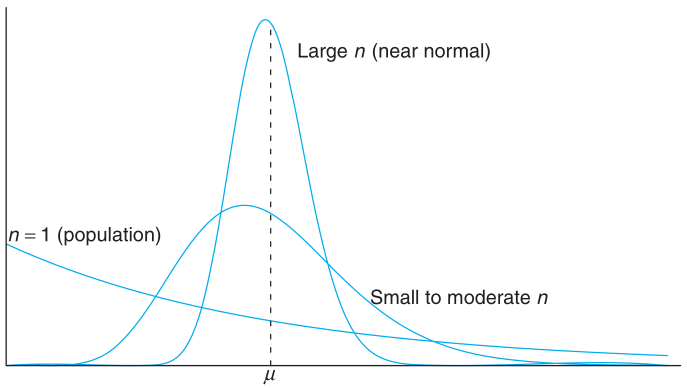
\includegraphics[width=0.8\textwidth]{CLT}
    \caption{Illustration of the Central Limit Theorem. Note that it shows how the mean of $\overline{X}$ remains $\mu$ for any sample size and the variance gets smaller as $n$ increases.}
    \label{fig:CLT}
\end{figure}
\begin{itemize}
    \item CLT is widely applicable -- works with any distribution as long as observations have same probability distributions with finite variance
    \item variance of mean shrinks with $ \sqrt{n} $ -- average becomes more accurate with a bigger sample
\end{itemize}

\subsection{Sampling Distribution of the Difference Between Two Means}
\begin{theorem}
    If independent samples of size $n_1$ and $n_2$ are drawn at random from two populations with means $\mu_1$ and $\mu_2$ and variances $\sigma_1^2$ and $\sigma_2^2$, then the sampling distribution of the differences of means, $\overline{X}_1-\overline{X}_2$, is approximately normally distributed with mean and variance given by 
    \begin{gather*}
        \mu_{\overline{X}_1-\overline{X}_2} = \mu_1-\mu_2 \quad \text{and} \quad \sigma_{\overline{X}_1-\overline{X}_2}^2 = \frac{\sigma_1^2}{n_1} + \frac{\sigma_2^2}{n_2}
    .\end{gather*}
    Therefore,
    \begin{gather*}
        Z = \frac{(\overline{X}_1-\overline{X}_2)-(\mu_1-\mu_2)}{\sqrt{(\sigma_1^2 / n_1) + (\sigma_2^2 / n_2)} }
    \end{gather*}
    is approximately a standard normal variable.
\end{theorem}



\section{Sampling Distribution of Variance}
\begin{theorem}
    If $S^2$ is the variance of a random sample of size $n$ taken from a normal population having the variance $\sigma^2$, then the statistic 
    \begin{gather*}
        \chi^2 = \frac{(n-1)S^2}{\sigma^2} = \sum_{i=1}^{n} \frac{(X_i-\overline{X})}{\sigma^2}
    .\end{gather*}
    has a chi-squared distribution with $\nu = n-1$.
\end{theorem}
\begin{figure}[h]
    \centering
    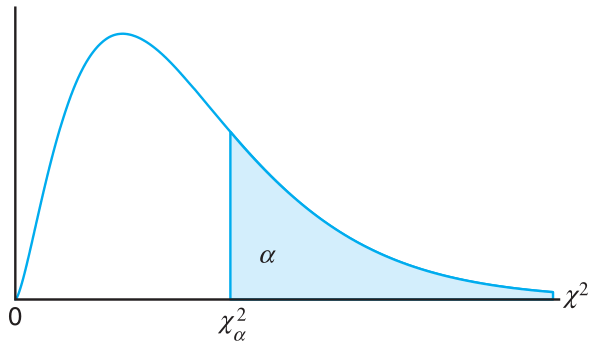
\includegraphics[width=0.6\textwidth]{chiSquaredSampling}
    \caption{The chi-squared disribution. We let $\chi_\alpha^2$ represent the $ \chi^2$ value above which we find an area of $\alpha$.}
    \label{fig:}
\end{figure}

\subsection{Degrees of Freedom as a Measure of Sample Information}
\begin{itemize}
    \item recall that
        \begin{gather*}
            \sum_{i=1}^{n} \frac{(X_i-\mu)^2}{\sigma^2}
        \end{gather*}
        has a chi-squared distribution with $n$ \textit{degrees of freedom} while the RV 
        \begin{gather*}
            \frac{(n-1)S^2}{\sigma^2} = \sum_{i=1}^{n} \frac{(X_i-\overline{X})}{\sigma^2}
        .\end{gather*}
        has a chi-squared distribution with $n-1$ \textit{degrees of freedom} 
    \item this is because when $\mu$ is not known, i.e. when we are considering the distribution of 
        \begin{gather*}
            \sum_{i=1}^{n} \frac{(X_i-\overline{X})}{\sigma^2}
        .\end{gather*}
        there is 1 less degree of freedom since a degree of freedom is lost in the estimation of $\mu$ (when $\mu$ is replaced by $\overline{x}$)
    \item when $\mu$ is known, there are $n$ degrees of freedom, or independent \textit{pieces of information}, in a random sample from a normal distribution
    \item when data (values in the sample) are used to compute the mean, there is 1 less DOF, 1 less piece of information, used to estimate $\sigma^2$
\end{itemize}



\section{\textit{t}-Distribution}
\begin{itemize}
    \item CLT is for making inferences about the mean $\mu$ assuming variance $\sigma^2$ is known
    \item \textit{t}-distribution is for when $\sigma^2$ is not known
    \item consider the statistic 
        \begin{gather*}
            T = \frac{\overline{X}-\mu}{S / \sqrt{n} }
        .\end{gather*}
        where
        \begin{gather*}
            S = \sqrt{\frac{1}{n-1}\sum_{i=1}^{n} (X_i-\overline{X})^2} 
        .\end{gather*}
    \item if sample size is large ($n \ge 30$), $S$ is close to $\sigma$, and $T$ follows a normal distribution
    \item if sample size is smaller, the values of $S^2$ fluctuate considerably and the disribution of $T$ deviates much more from the standard normal distribution
    \item the \textit{t}-distribution is much more accurate in this case
\end{itemize}
\begin{definition}
    \textbf{\textit{t}-distribution}:
    \begin{gather*}
        h(t) = \frac{\Gamma [(v+1) / 2]}{\Gamma (v / 2) \sqrt{\pi v}} \left( 1 + \frac{t^2}{v} \right)^{-(v+1) / 2} , \quad -\infty < t < \infty
    .\end{gather*}
\end{definition}
\begin{itemize}
    \item if $X_1, \ldots, X_n$ are independent RVs that are all normal with mean $\mu$ and standard deviation $\sigma$, and 
        \begin{gather*}
            \overline{X} = \frac{1}{n}\sum_{i=1}^{n} X_i \quad \text{and} \quad S^2 = \frac{1}{n-1}\sum_{i=1}^{n} (X_i-\overline{X})^2
        ,\end{gather*}
        then the RV $T = \frac{\overline{X}-\mu}{S / \sqrt{n} }$ has a \textit{t}-distribution with $v=n-1$ degrees of freedom
    \item intuition behind the \textit{t}-distribution: 
        \begin{itemize}
            \item if we knew $\sigma$, we'd have a normal distribution
            \item instead we only have estimate $S^2$ -- less information, so we expect more variability
        \end{itemize}
    \item variance of $T$ depends on the sample size $n$ and is always greater than 1 
    \item in the limit that sample size $n \to \infty$ and subsequently $v \to \infty$, the \textit{t}-distribution becomes the standard normal distribution
\end{itemize}
\begin{figure}[h]
    \centering
    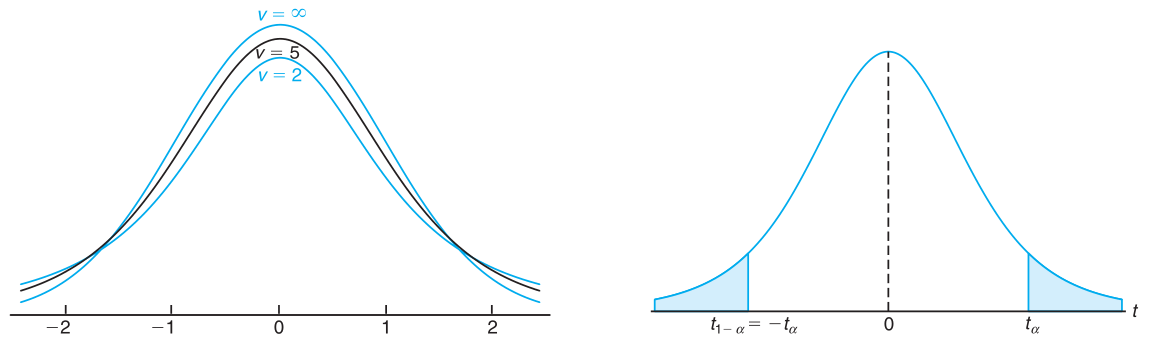
\includegraphics[width=0.8\textwidth]{tDistribution}
    \caption{Illustration of the \textit{t}-distribution. We let $t_\alpha$ represent the $t$-value above which we find an area equal to $\alpha$.}
    \label{fig:tDistribution}
\end{figure}


\section{\textit{F}-Distribution}
\begin{itemize}
    \item define a statistic $F$ to be the ratio of two independent chi-squared RVs $U$ and $V$, each divided by its number of degrees of freedom, $v_1$ and $v_2$:
        \begin{gather*}
            F = \frac{U / v_1}{V / v_2}
        .\end{gather*}
\end{itemize}
\begin{definition}
    \textbf{\textit{F}-distribution}: sampling distribution of $F$ is given by
    \begin{gather*}
        h(f) =
        \begin{cases}
            \frac{\Gamma[(v_1+v_2) / 2](v_1 / v_2)^{v_1 / 2}}{\Gamma(v_1 / 2) \Gamma(v_2 / 2)} \frac{f^{(v_1 / 2)-1}}{(1+v_1f / v_2)^{(v_1+v_2) / 2}} , & f > 0 \\
            0, & f \le 0
        \end{cases}
    .\end{gather*}
\end{definition}
\begin{figure}[h]
    \centering
    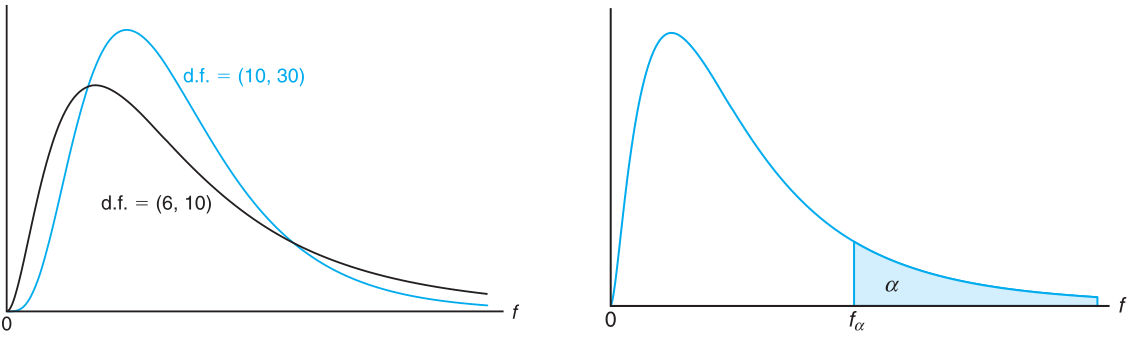
\includegraphics[width=0.8\textwidth]{fDistribution}
    \caption{Typical \textit{F}-distributions. We let $f_\alpha$ be the $f$-value above which we find an area equal to $\alpha$.}
    \label{fig:fDistribution}
\end{figure}

\subsection{The \textit{F}-Distribution with Two Sample Variances}
\begin{theorem}
    If $S_1^2$ and $S_2^2$ are the variances of independent random samples of size $n_1$ and $n_2$ taken from normal populations with variances $\sigma_1^2$ and $\sigma_2^2$, then
        \begin{gather*}
            F = \frac{S_1^2 / \sigma_1^2}{S_2^2 / \sigma_2^2} = \frac{\sigma_2^2 S_1^2}{\sigma_1^2 S_2^2}
        .\end{gather*}
        has an \textit{F}-distribution with $v_1 = n_1 - 1$ and $v_2 = n_2 - 1$ degrees of freedom
\end{theorem}



\section{Quantile and Probability Plots}
\begin{itemize}
    \item quantile plots depict (in sample form) the cumulative distribution function
\end{itemize}
\begin{definition}
    A \textbf{quantile} of a sample, denoted by $q(f)$, is a value for which a specified fraction of $f$ of the data values is less than or equal to $q(f)$.
\end{definition}
\begin{itemize}
    \item a \textbf{quantile plot} plots $q(f)$ versus $f$, where $q(f)$ is on the y-axis
    \item to sketch:
        \begin{itemize}
            \item rank sample in increasing order, $x_1, \ldots, x_n$
            \item for each data point $i = 1, \ldots, n$, plot 
                \begin{gather*}
                    \left( \frac{i-3 / 8}{n + 1 / 4}, x_i \right) 
                .\end{gather*}
        \end{itemize}
        \begin{figure}[h]
            \centering
            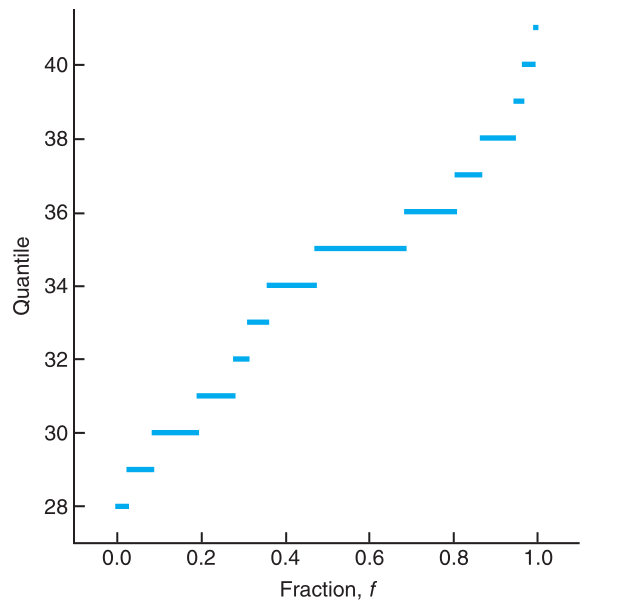
\includegraphics[width=0.8\textwidth]{quantilePlot}
            \caption{Example of a quantile plot.}
            \label{fig:quantilePlot}
        \end{figure}
    \item notice in Figure \ref{fig:quantilePlot}:
        \begin{itemize}
            \item $q(0.5)$ is the sample median
            \item lower quartile (25th percentile) is $q(0.25)$ 
            \item upper quartile (75th percentile) is $q(0.75)$ 
            \item flat areas indicate clusters of data 
            \item steep areas indicate sparsity of data
        \end{itemize}
\end{itemize}

\subsection{Normal Quantile-Quantile Plot}
\begin{itemize}
    \item we often want to know how close data is to a normal distribution since we understand normal distributions very well and many tools ($t$ and $F$ distributions) assume normality
    \item the expression for the quantile of a normal distribution is very complicated but can be approximated as 
        \begin{gather*}
            q_{\mu,\sigma}(f) = \mu + \sigma(4.91(f^{0.14} - (1-f)^{0.14}))
        .\end{gather*}
\end{itemize}
\begin{definition}
    \textbf{Normal quantile-quantile plot}: a plot of $y_{(i)}$ (ordered observations) against $q_{0,1}(f_i)$, where $f_i = \frac{i-3 / 8}{n + 1 / 4}$.
\end{definition}
\begin{itemize}
    \item if the curve is straight, the data is roughly normal
\end{itemize}
\begin{figure}[h]
    \centering
    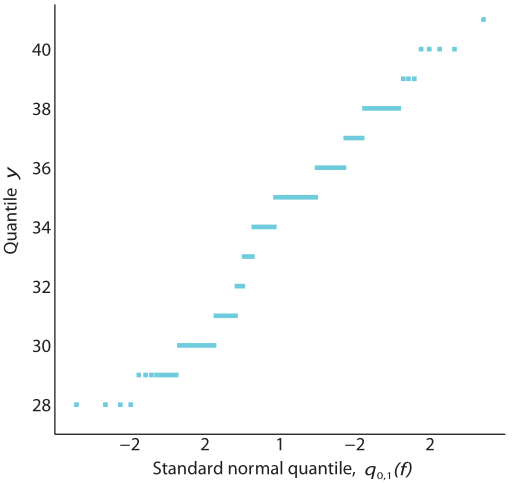
\includegraphics[width=0.8\textwidth]{normalQQPlot}
    \caption{Example of a normal quantile-quantile plot.}
    \label{fig:normalQQPlot}
\end{figure}





\newpage
\part{Estimation}

\section{Classical Methods of Estimation}
\begin{itemize}
    \item in general, given a sample, we write 
        \begin{itemize}
            \item $\theta$ is the true parameter of the population (like $\mu$)
            \item $ \hat{\theta}$ is the observed value from the sample (like $\overline{x}$)
            \item $\hat{\Theta}$ is the sample statistic (like $\overline{X}$)
        \end{itemize}
\end{itemize}
\begin{definition}
    A \textbf{point estimate} of some population parameter $\theta$ is a single value $\hat{\theta}$ of a statistic $\hat{\Theta}$.
    \begin{itemize}
        \item for example: the value $\overline{x}$ of the statistic $\overline{X}$, computed from a sample of size $n$, is a point estimate of the population parameter $\mu$.
    \end{itemize}
\end{definition}

\subsection{Unbiased Estimator}
\begin{definition}
    A statistic $\hat{\Theta}$ is said to be an \textbf{unbiased estimator} of the parameter $\theta$ if 
    \begin{gather*}
        \mu_{\hat{\Theta}} = E(\hat{\Theta}) = \theta
    .\end{gather*}
\end{definition}

\subsection{Variance of a Point Estimator}
\begin{definition}
    Considering all possible unbiased estimators of some parameter $\theta$, the one with the smallest variance is called the \textbf{most efficient estimator} of $\theta$.
\end{definition}
\begin{figure}[h]
    \centering
    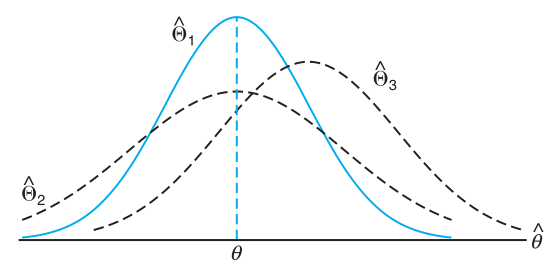
\includegraphics[width=0.8\textwidth]{unbiasedEstimator}
    \caption{Sampling distributions of different estimators of $\theta$.}
    \label{fig:unbiasedEstimator}
\end{figure}

\subsection{Interval Estimation}
\begin{itemize}
    \item a point estimate $\hat{\theta}$ is rarely exactly $\theta$ 
    \item it's useful to have an interval, $\hat{\theta_L} \le \theta \le \hat{\theta_U}$
    \item $\hat{\theta_L}$ and $\hat{\theta_U}$ depend on the value of the statistic $\hat{\Theta}$ for a particular sample and also on the sampling distribution of $\hat{\Theta}$
    \item we want to make a statement of the form 
        \begin{gather*}
            P(\hat{\Theta_L} < \theta < \hat{\Theta_U}) = 1 - \alpha
        \end{gather*}
        for $0 < \alpha < 1$
    \item the interval $\hat{\theta_L} \le \theta \le \hat{\theta_U}$, computed from the selected sample, is called a $100(1-\alpha)\%$ \textbf{confidence interval} 
        \begin{itemize}
            \item e.g. if $\alpha = 0.05$, we have a 95\% confidence interval 
        \end{itemize}
    \item the fraction $1-\alpha$ is called the \textbf{confidence coefficient} or \textbf{degree of confidence}
    \item the endpoints of the interval are called the lower and upper \textbf{confidence limits} 
\end{itemize}


\section{Single Sample: Estimating the Mean}
\begin{itemize}
    \item Setup:
        \begin{itemize}
            \item $n$ samples
            \item observed mean $\overline{x}$ 
            \item known variance $\sigma^2$ 
            \item and the statistic $Z = \frac{\overline{X}-\mu}{\sigma / \sqrt{n} }$
        \end{itemize}
    \item then 
        \begin{gather*}
            1 - \alpha = P(-z_{\alpha / 2} \le Z \le z_{\alpha / 2}),
        \end{gather*}
        where
        \begin{gather*}
            z_{\beta} = - \Phi^{-1}(\beta)
        \end{gather*}
        and
        \begin{gather*}
            \Phi(x) = \frac{1}{\sqrt{2\pi} } \int_{-\infty}^{x} e^{-t^2 / 2} dt
        .\end{gather*}
\end{itemize}
\begin{theorem}
    If $\overline{x}$ is used as an estimate of $\mu$, we can be $100(1-\alpha)\%$ confident that the error will not exceed $z_{\alpha / 2}\frac{\sigma}{\sqrt{n} }$.
    \begin{itemize}
        \item i.e.
            \begin{gather*}
                \overline{X}_L = \overline{X} - z_{\alpha / 2} \frac{\sigma}{\sqrt{n} } \quad \text{and} \quad \overline{X}_U = \overline{X} + z_{\alpha / 2} \frac{\sigma}{\sqrt{n} }
            .\end{gather*}
    \end{itemize}
\end{theorem}
\begin{theorem}
    If $\overline{x}$ is used as an estimate of $\mu$, we can be $100(1-\alpha)\%$ confident that the error will not exceed a specificed amount $e$ when the sample size is 
    \begin{gather*}
        n = \left( \frac{z_{\alpha / 2}\sigma}{e} \right) ^2
    .\end{gather*}
\end{theorem}

\subsection{One-Sided Confidence Intervals}
\begin{itemize}
    \item if we want a confidence interval of the form
        \begin{gather*}
            1-\alpha = P(Z \le z_\alpha)
        \end{gather*}
        we set
        \begin{gather*}
            z_\alpha = -\Phi^{-1}(\alpha)
        .\end{gather*}
    \item then:
        \begin{gather*}
            \overline{X}_U = \overline{X} + z_\alpha \frac{\sigma}{\sqrt{n} }
        .\end{gather*}
\end{itemize}

\subsection{Estimates with Unknown $\sigma$}
\begin{itemize}
    \item samples from normal distribution with unknown $\sigma$ and any $n$, we use \textit{t}-distribution
\end{itemize}
\begin{theorem}
    If $\overline{x}$ and $s$ are the mean and standard deviation of a random sample from a normal population with an unknown variance $\sigma^2$, a $100(1-\alpha)\%$ confidence interval for $\mu$ is
    \begin{gather*}
        \overline{x}-t_{\alpha / 2} \frac{s}{\sqrt{n} } < \mu < \overline{x}+t_{\alpha / 2} \frac{s}{\sqrt{n} }
    \end{gather*}
    where $t_{\alpha / 2}$ is the \textit{t}-value with $v=n-1$ degrees of freedom, leaving an area of $\alpha / 2$ to the right.
\end{theorem}
\begin{itemize}
    \item one-sided confidence intervals (upper and lower $100(1-\alpha)\%$ confidence intervals) for $\mu$ with unknown $\sigma$ are
        \begin{gather*}
            \overline{x}+t_{\alpha} \frac{s}{\sqrt{n} } \quad \text{and} \quad \overline{x}-t_{\alpha} \frac{s}{\sqrt{n} }
        .\end{gather*}
\end{itemize}


\section{Standard Error of a Point Estimate}
\begin{itemize}
    \item given samples $X_1, \ldots, X_n$ drawn from an unknown distribution with variance $\sigma$ 
    \item as $n \to \infty$, the distribution of $Z = \frac{\overline{X}-\mu}{\sigma / \sqrt{n} }$ approaches $n(z;0,1)$, the standard normal
    \item this implies that the standard deviation of $Z$ is around $\frac{\sigma}{n}$ 
\end{itemize}
\begin{definition}
    The \textbf{standard error} of an estimator is its standard deviation.
    \begin{itemize}
        \item e.g. the standard of error of $\overline{X}$ is $\sigma / \sqrt{n} $
        \item recall the $100(1-\alpha)\%$ confidence intervals for the mean:
            \begin{gather*}
                \overline{x} \pm z_{\alpha / 2} \frac{\sigma}{\sqrt{n}} \quad \text{is written as} \quad \overline{x} \pm z_{\alpha / 2} \text{s.e.} (\overline{x})
            \end{gather*}
            where "s.e." is the standard error
    \end{itemize}
\end{definition}
\begin{itemize}
    \item the width of confidence intervals depends on the confidence and the standard error
\end{itemize}


\section{Prediction Intervals}
\begin{itemize}
    \item so far we've been give samples and $\overline{X}$ and characterized the error/uncertainty of $\overline{X}$ 
    \item we now want to predict the value of a future observation
    \item suppose we have normal samples $X_1, \ldots, X_n$, each with known variance $\sigma$ and a sample mean of $\overline{X}$ 
    \item $\overline{X}$ is a good point estimate of a single new sample $ X_0$
    \item the error of the point estimate is $X_0 - \overline{X}$ 
    \item due to independence, the variance of the error is $\sigma^2 + \sigma^2 / n$
    \item we define the statistic
        \begin{gather*}
            Z = \frac{X_0 - \overline{X}}{\sigma \sqrt{1 + 1 / n} }
        .\end{gather*}
    \item the distribution of $Z$ is $n(z;0,1)$ 
    \item therefore we can write the probability statement
        \begin{gather*}
            1-\alpha = P(-z_{\alpha / 2} \le Z \le z_{\alpha / 2})
        .\end{gather*}
\end{itemize}
\begin{theorem}
    For a normal distribution of measurements with unknown mean $\mu$ and known variance $\sigma^2$, a $100(1-\alpha)\%$ \textbf{prediction interval} of a future observation $x_0$ is
    \begin{gather*}
        \overline{x} - z_{\alpha / 2} \sigma \sqrt{1+1 / n} < x_0 < \overline{x} + z_{\alpha / 2} \sigma \sqrt{1+1 / n}
    ,\end{gather*}
    where $z_{\alpha / 2}$ is the $z$-value leaving an area of $\alpha / 2$ to the right.
\end{theorem}
\begin{theorem}
    For a normal distribution of measurements with unknown mean $\mu$ and unknown variance $\sigma^2$, a $100(1-\alpha)\%$ \textbf{prediction interval} of a future observation $x_0$ is
    \begin{gather*}
        \overline{x} - t_{\alpha / 2} s \sqrt{1+1 / n} < x_0 < \overline{x} + t_{\alpha / 2} s \sqrt{1+1 / n}
    ,\end{gather*}
    where $t_{\alpha / 2}$ is the $t$-value with $v=n-1$ degrees of freedom, leaving an area of $\alpha / 2$ to the right.
\end{theorem}
\begin{itemize}
    \item \textbf{outlier detection}: if a new observation is outside the prediction interval, we can declare it an outlier
\end{itemize}


\section{Tolerance Limits}
\begin{itemize}
    \item we want to define bounds that cover a fixed proportion of the measurements
\end{itemize}
\begin{definition}
    For a normal distribution of measurements with unknown mean $\mu$ and unknown standard deviation $\sigma$, \textbf{tolerance limits} are given by $\overline{x} \pm ks$, where $k$ is determined such that one can assert with $100(1-\gamma)\%$ confidence that the given limits contain at least the proportion of $1-\alpha$ of the measurements. 
    \begin{itemize}
        \item values of $k$ given in a provided table
    \end{itemize}
\end{definition}

\subsection{Comparison of Intervals}
\begin{itemize}
    \item Confidence Intervals:
        \begin{itemize}
            \item setup: independent observations of RVs, $x_1, \ldots, x_n$, and the mean is $\overline{x}=\frac{1}{n}\sum_{i=1}^{n} x_i$ 
            \item there is a $100(1-\alpha)\%$ chance the true mean $\mu$ is in an interval around $\overline{x}$
            \item use CLT to compute interval when we know $\sigma$ for each observation or $n$ is large 
            \item use $t$-distribution when $\sigma$ is unknown
        \end{itemize}
    \item Prediction Intervals:
        \begin{itemize}
            \item same setup 
            \item $100(1-\alpha)\%$ chance the next observation $x_0$ is in an interval around $\overline{x}$ 
            \item compute from $t$ or normal distribution
        \end{itemize}
    \item Tolerance Limits:
        \begin{itemize}
            \item same setup 
            \item $100(1-\gamma)\%$ of measurements will be in an interval $\overline{x} \pm ks$ 
            \item compute from table
        \end{itemize}
\end{itemize}


\section{Two Samples: Estimating the Difference between Two Means}
\begin{itemize}
    \item if we have two populations with means $\mu_1$ and $\mu_2$ and variances $\sigma^2_1$ and $\sigma_2^2$ 
    \item then a point estimator of the difference between $\mu_1$ and $\mu_2$ is given by the statistic $\overline{X}_1 - \overline{X}_2$ 
    \item therefore to obtain a point estimate of $\mu_1 - \mu_2$, we select independent random sample from each population of sizes $ n_1$ and $n_2$ and compute $\overline{x}_1 - \overline{x}_2$ (the difference of the sample means)
    \item the sampling distribution of $\overline{X}_1 - \overline{X}_2$ is approximately normally distributed with mean $\mu_{\overline{X}_1-\overline{X}_2} = \mu_1 - \mu_2$ and standard deviation $\sigma_{\overline{X}_1-\overline{X}_2}=\sqrt{\sigma_1^2 / n_1 + \sigma_2^2 / n_2}$
    \item therefore, we define a standard normal variable 
        \begin{gather*}
            Z = \frac{(\overline{X}_1-\overline{X}_2)-(\mu_1-\mu_2)}{\sqrt{\sigma_1^2 / n_1 + \sigma_2^2 / n_2}}
        \end{gather*}
    \item and assert that 
        \begin{gather*}
            P(-z_{\alpha / 2} < Z < z_{\alpha / 2}) = 1 - \alpha
        .\end{gather*}
\end{itemize}
\begin{theorem}
    \textbf{Confidence Interval for $\mu_1-\mu_2$, Known Variances}: If $\overline{x}_1$ and $\overline{x}_2$ are means of independent random samples of sizes $n_1$ and $n_2$ from populations with known variances $\sigma_1^2$ and $\sigma_2^2$, a $100(1-\alpha)\%$ confidence interval for $\mu_1 - \mu_2$ is given by
    \begin{gather*}
        (\overline{x}_1-\overline{x}_2) - z_{\alpha / 2} \sqrt{\frac{\sigma_1^2}{n_1} + \frac{\sigma_2^2}{n_2}} < \mu_1 - \mu_2 < (\overline{x}_1-\overline{x}_2) + z_{\alpha / 2} \sqrt{\frac{\sigma_1^2}{n_1} + \frac{\sigma_2^2}{n_2}}
    \end{gather*}
    where $z_{\alpha / 2}$ is the $z$-value leaving an area of $\alpha / 2$ to the right.
\end{theorem}

\subsection{Two Samples with Unknown Variance}
\subsubsection{Equal Variances}
\begin{definition}
    \textbf{Pooled Estimate of Variance}: the sample size-weighted average of $S_1^2$ and $S_2^2$ 
    \begin{gather*}
        S_p^2 = \frac{(n_1-1)S_1^2 + (n_2-1)S_2^2}{n_1 + n_2 - 2}
    .\end{gather*}
\end{definition}
\begin{itemize}
    \item define the statistic 
        \begin{gather*}
            T = \frac{(\overline{X}_1 - \overline{X}_2) - (\mu_1 - \mu_2)}{S_p \sqrt{1 / n_1 + 1 / n_2}}
        .\end{gather*}
    \item then $T$ has the $t$-distribution with $v = n_1 + n_2 - 2$ degrees of freedom
    \item we have 
        \begin{gather*}
            P(-t_{\alpha/2} < T < t_{\alpha / 2}) = 1- \alpha
        .\end{gather*}
\end{itemize}
\begin{theorem}
    \textbf{Confidence Interval for $\mu_1 - \mu_2$, Equal but Unknown Variances}: a $100(1-\alpha)\%$ confidence interval for $\mu_1-\mu_2$ is given by 
    \begin{gather*}
        (\overline{x}_1 - \overline{x}_2) - t_{\alpha / 2} s_p \sqrt{1 / n_1 + 1 / n_2} < \mu_1 - \mu_2 < (\overline{x}_1 - \overline{x}_2) + t_{\alpha / 2} s_p \sqrt{1 / n_1 + 1 / n_2}
    ,\end{gather*}
    where $s_p$ is the pooled estimate of the population standard deviation and $t_{\alpha / 2}$ is the $t$-value with $v=n_1 + n_2 -2$ degrees of freedom, leaving an area of $\alpha / 2$ to the right.
\end{theorem}

\subsubsection{Different Variances}
\begin{itemize}
    \item if the variances are unknown and different, we use the statistic 
        \begin{gather*}
            T' = \frac{(\overline{X}_1-\overline{X}_2) - (\mu_1 - \mu_2)}{\sqrt{S_1^2 / n_1 + S_2^2 / n_2}}
        .\end{gather*}
    \item then $T'$ approximately has a $t$-distribution with 
        \begin{gather*}
            v = \frac{(s_1^2 / n_1 + s_2^2 / n_2)^2}{(s_1^2 / n_1)^2 / (n_1 -1) + (s_2^2 / n_2)^2 / (n_2-1)}
        \end{gather*}
        degrees of freedom
\end{itemize}


\section{Paired Observations}
\begin{itemize}
    \item previously we considered two sample populations of different sizes and all measurements were independent
    \item now we consider two sample populations of the same size and pairs of observations have one measurement from each population
        \begin{itemize}
            \item e.g. measuring before and after observations on $n$ people -- each "before" measurement is paired with an "after" measurement
        \end{itemize}
    \item consider paired samples $(X_i, Y_i), i = 1, \ldots, n$ with statistics $\mu_X, \sigma_X, \ldots$ (same for $Y_i$'s)
    \item we are interested in the difference $D_i = X_i - Y_i$
    \item the variance of the difference: 
         \begin{gather*}
            \text{var}(D_i) = \text{var}(X_i - Y_i) = \sigma_X^2 + \sigma_Y^2 - 2 \text{cov}(X_i, Y_i)
        .\end{gather*}
    \item we expect $\text{cov}(X_i, Y_i) \ge 0$, e.g. the before and after weights for one person is likely both above $\mu_X$ and $\mu_Y$
    \item pairing helps reduce variance
    \item we can then apply usual CLT or $t$-distribution confidence intervals to sample $D_i$
\end{itemize}


\section{Single Sample: Estimating a Proportion}
\begin{itemize}
    \item a point estimator of the proportion $p$ in a binomial experiment is given by the staistic $\hat{P} = X / n$ 
    \item $X$ represents the number of successes in $n$ trials
    \item the sample proportion $\hat{p} = x / n$ is used as the point estimate of the parameter $p$
    \item by CLT, for $n$ sufficiently large, $\hat{P}$ is approximately normally distributed with mean $p$ and variance $\frac{pq}{n}$ 
    \item we can use the statistic
        \begin{gather*}
            Z=\frac{\hat{P}-p}{\sqrt{pq / n}}
        .\end{gather*}
\end{itemize}
\begin{theorem}
    \textbf{Large Sample Confidence Intervals for $p$}: If $\hat{p}$ is the proportion of successes in a random sample of size $n$ and $\hat{q} = 1- \hat{p}$, an approximate $100(1-\alpha)\%$ confidence interval for the binomial parameter $p$ is given by (method 1)
    \begin{gather*}
        \hat{p} - z_{\alpha / 2}\sqrt{\frac{\hat{p}\hat{q}}{n}} < p < \hat{p} + z_{\alpha / 2}\sqrt{\frac{\hat{p}\hat{q}}{n}}
    \end{gather*}
    or by the limits (method 2)
    \begin{gather*}
        \frac{\hat{p} + \frac{z_{\alpha / 2}^2}{2n}}{1 + \frac{z_{\alpha / 2}^2}{n}} \pm \frac{z_{\alpha / 2}}{1 + \frac{z_{\alpha / 2}^2}{n}} \sqrt{\frac{\hat{p}\hat{q}}{n} + \frac{z_{\alpha / 2}^2}{4n^2}}
    .\end{gather*}
\end{theorem}
\begin{theorem}
    If $\hat{p}$ is used as an estimate of $p$, we can be $100(1-\alpha)\%$ confident that the error will not exceed $z_{\alpha / 2}\sqrt{\hat{p}\hat{q} / n} $.
\end{theorem}

\subsection{Choice of Sample Size}
\begin{itemize}
    \item suppose we want to be $100(1-\alpha)\%$ confident that the error is less than some specified amount $e$
\end{itemize}
\begin{theorem}
    If $\hat{p}$ is used as an estimate of $p$, we can be $100(1-\alpha)\%$ confident that the error will be less than a specified amount $e$ when the sample size is approximately 
    \begin{gather*}
        n = \frac{z_{\alpha / 2}^2 \hat{p} \hat{q}}{e^2}
    .\end{gather*}
\end{theorem}
\begin{itemize}
    \item but there's a catch: $\hat{p}$ depends on $n$
    \item if we want a safe lower bound for  $n$ :
\end{itemize}
\begin{theorem}
    If $\hat{p}$ is used as an estimate of $p$, we can be \textbf{at least} $100(1-\alpha)\%$ confident that the error will not exceed a specified amount $e$ when the sample size is 
    \begin{gather*}
        n = \frac{z_{\alpha / 2}^2}{4e^2}
    .\end{gather*}
\end{theorem}


\section{Single Sample: Estimating the Variance}
\begin{itemize}
    \item an interval estimate of $\sigma^2$ can be established using the statistic 
        \begin{gather*}
            X^2 = \frac{(n-1)S^2}{\sigma^2}
        .\end{gather*}
\end{itemize}
\begin{theorem}
    \textbf{Confidence Interval for $\sigma^2$}: If $s^2$ is the variance of a random sample of size $n$ from a normal population, a $100(1-\alpha)\%$ confidence interval for $\sigma^2$ is 
    \begin{gather*}
        \frac{(n-1)s^2}{\chi_{\alpha / 2}^2} < \sigma^2 < \frac{(n-1)s^2}{\chi_{1-\alpha / 2}^2}
    ,\end{gather*}
    where $ \chi_{\alpha / 2}^2$ and $ \chi_{1-\alpha / 2}^2$ are $\chi^2$-values with $v=n-1$ degrees of freedom, leaving areas of $\alpha / 2$ and $1-\alpha/2$ to the right.
\end{theorem}


\section{Maximum Likelihood Estimation}
\begin{itemize}
    \item so far, we've used intuitive sampling statistics:
        \begin{itemize}
            \item $\overline{X}$ for $\mu$, $S^2$ for $\sigma^2$, $\hat{P}$ for $p$
        \end{itemize}
    \item but sometimes it is not obvious what the proper estimator for parameters should be 
        \begin{itemize}
            \item e.g. degrees of freedom, $\alpha$ and $\beta$ in gamma distribution, etc.
        \end{itemize}
    \item one of the most important approaches to estimation in statistical inference: \textbf{method of maximum likelihood} 
\end{itemize}

\subsection{The Likelihood Function}
\begin{itemize}
    \item the method of maximum likelihood is that for which the likelihood function is maximized
    \item main philosophy: the reasonable estimator of a parameter based on sample information is the parameter value that produces the largest probability of obtaining the sample -- given a sample, what was the parameter value that most likely produced it
    \item the likelihood of a sample for a certain value of a parameter is simply the joint distribution of the random variables for a certain value of that parameter, i.e.
        \begin{gather*}
            P(X_1 = x_1, \ldots, X_n = x_n | \theta) = f(x_1, \theta)\ldots f(x_n, \theta)
        .\end{gather*}
\end{itemize}
\begin{definition}
    Given independent observations $x_1, x_2, \ldots, x_n$ from a probability density function (continuous case) or probability mass function (discrete case) $f(\bm{x};\theta)$, the maximum likelihood estimator (MLE) $\hat{\theta}$ is that which maximizes the \textbf{likelihood function} 
    \begin{gather*}
        L(x_1, x_2, \ldots, x_n; \theta) = \prod_{i=1}^{n} f(x_i, \theta)  = f(x_1, \theta)f(x_2,\theta)\ldots f(x_n, \theta)
    ,\end{gather*}
    i.e.
    \begin{gather*}
        \hat{\theta} = \max_{\theta} L(x_1, \ldots, x_n; \theta)
    .\end{gather*}
\end{definition}
\begin{itemize}
    \item it is often convenient to work with the natural log of the likelihood function in finding its maximum
    \item for example, given an RV $X$ with a gamma distribution and a sample $x_1, \ldots, x_n$, how can we estimate  $\alpha$ and $\beta$? 
    \item using MLE:
        \begin{gather*}
            \hat{\alpha} = \max_{\alpha} \prod_{i=1}^{n} f(x_i; \alpha, \beta) 
        ,\end{gather*}
        and same applies to $\beta$
\end{itemize}







\newpage
\part{Hypothesis Testing}

\section{Statiscal Hypotheses: General Concepts}
\begin{definition}
    \textbf{Statistical Hypothesis}: an assertion or conjecture concerning one or more populations (a special case of more general hypotheses)
\end{definition}
\begin{itemize}
    \item rejection of a hypothesis implies that the sample evidence refutes it -- there is a extremely small probability of obtaining the sample information observed if the hypothesis was true (therefore it isn't)
    \item typically, a contention is reached via a rejection of an opposing hypothesis
\end{itemize}

\subsection{The Null and Alternative Hypotheses}
\begin{itemize}
    \item \textbf{null hypothesis}: any hypothesis we wish to test, denoted by $ H_0$
    \item the rejection of $H_0$ leads to the acceptance of the \textbf{alternative hypothesis}, denoted by $H_1$ 
    \item the alternative hypothesis $H_1$ usually represents the \textit{question to be answered or the theory to be tested} (its specification is crucial)
    \item the null hypothesis nullifies or opposes the alternative hypothesis (they are often logical complements)
    \item a data analyst arrives at one of two conclusions:
        \begin{enumerate}
            \item \textbf{reject $H_0$} in favour of $H_1$ because of sufficient evidence in the data, or
            \item \textbf{fail to reject $H_0$} because of insufficient evidence in the data
        \end{enumerate}
    \item for example: innocent until proven guilty:
        \begin{itemize}
            \item $H_0$ is innocent, $H_1$ is guilty 
            \item if there is strong enough evidence pointing to guilty, we reject $H_0$ in favour of $H_1$
            \item if evidence is weak, we fail to reject $H_0$ 
            \item \textbf{key point}: we are not proving innocence, we are \textit{failing to reject} innocence
        \end{itemize}
    \item \textbf{hypothesis testing} is using confidence intervals and logic to draw these conclusions
\end{itemize} 



\section{Testing a Statistical Hypothesis}
\begin{definition}
    \textbf{Type I error}: rejection of the null hypothesis when it's actually true (false positive)
    \begin{itemize}
        \item \textbf{level of significance}: probability of committing a type I error
            \begin{gather*}
                \alpha = P(\text{type I error})
            .\end{gather*}
    \end{itemize}
\end{definition}
\begin{definition}
    \textbf{Type II error}: nonrejection of the null hypothesis when it's actually false (false negative)
    \begin{itemize}
        \item \textbf{level of significance}: probability of committing a type II error 
            \begin{gather*}
                \beta = P(\text{type II error})
            .\end{gather*}
    \end{itemize}
\end{definition}
\begin{itemize}
    \item the probability of committing both types of error can be reduced by increasing the sample size
\end{itemize}
\textbf{Example:} mean weight of male students in a college
\begin{itemize}
    \item our null and alternative hypotheses: $H_0$ is $\mu = 68$ kg, $H_1$ is $\mu \neq 68$ kg
    \item we encounter a first issue: $P(H_0) = P(\mu = 68) = 0$ 
        \begin{itemize}
            \item then $H_0$ will almost always be rejected
        \end{itemize}
    \item to solve this we use a \textbf{critical region} -- a range leading to rejection of $H_0$:
        \begin{itemize}
            \item if $67 < \overline{x} < 69$, don't reject $H_0$
            \item critical region is the complement of [67, 69]
                \begin{figure}[H]
                    \centering
                    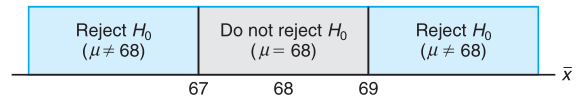
\includegraphics[width=0.8\textwidth]{criticalRegion}
                    \caption{Critical region shown in blue.}
                    \label{fig:criticalRegion}
                \end{figure}
        \end{itemize}
    \item we now calculate the probabilties of committing type I and type II errors
    \item assume sample size of $n=36$
    \item we assume that standard deviation of the population of weights is $\sigma = 3.6$
         \begin{itemize}
            \item for larger samples, we may substitute $s$ for $\sigma$ if no other estimate of $\sigma$ is available
        \end{itemize}
    \item our decision statistic will be $\overline{X}$, the most efficient estimator of $\mu$ 
    \item from the CLT, we know the sampling distribution of $\overline{X}$ is approximately normal with standard deviation $\sigma_{\overline{X}} = \sigma / \sqrt{n} = 3.6 / 6 = 0.6$
    \item the probability of committing a type I error is given by 
        \begin{gather*}
            \alpha = P(\overline{X} < 67) + P(\overline{X} > 69) \quad \text{when $\mu = 68$}
        .\end{gather*}
        \begin{figure}[h]
            \centering
            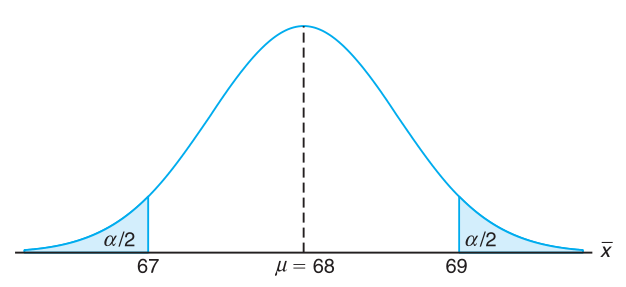
\includegraphics[width=0.8\textwidth]{type1ErrorProb}
            \caption{Probability of a type I error.}
            \label{fig:type1ErrorProb}
        \end{figure}
    \item converting to $z$-values and looking at tables for normal distribution, we find that $\alpha = 0.0950$ 
    \item interpretation: 9.5\% of all samples of size 36 would lead us to reject $\mu=68$ kg when in fact it is true 
    \item to reduce $\alpha$, we can increase sample size or widen the fail-to-reject region
        \begin{itemize}
            \item if we increase sample size to 64, then repeating the calculations, we obtain $\alpha=0.0264$
        \end{itemize}
    \item but reduction in $\alpha$ is not sufficient by itself to guarantee good testing procedure, we must also evaluate $\beta$ for various alternative hypotheses
    \item if it's important to reject $H_0$ when the true mean is some value $\mu \ge 70$ or $\mu \le 66$, then the probability of committing a type II error should be calculated for alternatives $\mu = 66$ and $\mu = 70$
         \begin{itemize}
            \item due to symmetry, it's only necessary to consider one case
        \end{itemize}
    \item a type II error occurs when $67 < \overline{x} < 69$ when $H_1$ is true: 
        \begin{gather*}
            \beta = P(67 \le \overline{X} \le 69 \; \text{when} \; \mu = 70)
        .\end{gather*}
        \begin{figure}[h]
            \centering
            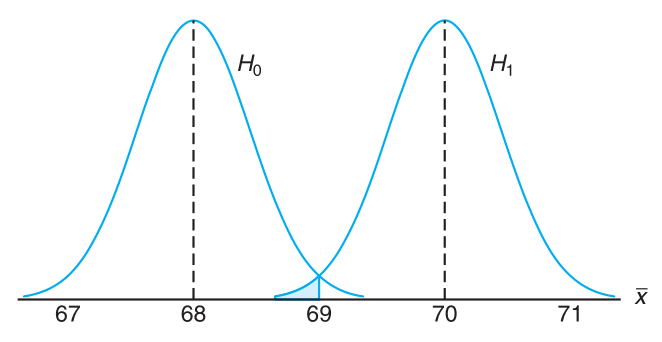
\includegraphics[width=0.8\textwidth]{type2ErrorProb}
            \caption{Probability of type II error for testing $\mu = 68$ versus $\mu = 70$.}
            \label{fig:type2ErrorProb}
        \end{figure}
    \item by calculating $z$-values and looking at tables, we obtain $\beta = 0.0132$ (same result if the true value of $\mu$ was 66)
    \item again, the value of $\beta$ can be decreased if sample size $n$ is increased
    \item the probability of committing a type II error increases rapidly when the true value of $\mu$ approaches (but is not equal to) the hypothesized value
        \begin{itemize}
            \item for example, if the alternative hypothesis $\mu=68.5$ is true:
                \begin{figure}[H]
                    \centering
                    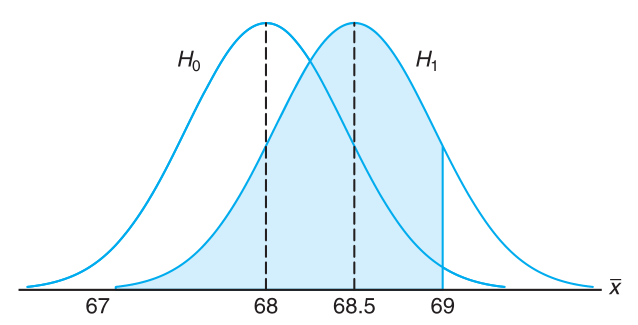
\includegraphics[width=0.8\textwidth]{type2ErrorProbClose}
                    \caption{Probability of type II error for testing $\mu=68$ vs $\mu = 68.5$}
                    \label{fig:type2ErrorProbClose}
                \end{figure}
        \end{itemize}
\end{itemize}
\begin{theorem}
    \textbf{Important Properties of a Hypothesis Test}:
    \begin{enumerate}
        \item type I and type II error are related (decrease in probability of one generally results in an increase in the probability of the other)
        \item size of the critical region (and therefore the probability of committing a type I error) can always be reduced by adjusting the critical values
        \item increase in sample size will reduce $\alpha$ and $\beta$ 
        \item if the null hypothesis $H_0$ is false, $\beta$ is maximized when the true value of a parameter approaches the hypothesized value (the greater the distance between the true and hypothesized value, the smaller it will be)
    \end{enumerate}
\end{theorem}
\begin{definition}
    \textbf{Power} of a test: the probability of rejecting $H_0$ given that a specific alternative is true.
    \begin{itemize}
        \item computed as $1-\beta$
    \end{itemize}
\end{definition}

\subsection{One- and Two-Tailed Tests}
\begin{itemize}
    \item \textbf{one-tailed test}: a test of a statistical hypothesis where the alternative is \textbf{one sided}
        \begin{itemize}
            \item for example:
                \begin{gather*}
                    H_0: \theta = \theta_0 \\ 
                    H_1: \theta > \theta_0
                .\end{gather*}
        \end{itemize}
    \item \textbf{two-tailed test}: a test of a statistical hypothesis where the alternative is \textbf{two sided}
        \begin{itemize}
            \item for example:
                \begin{gather*}
                    H_0: \theta = \theta_0 \\ 
                    H_1: \theta \neq \theta_0
                .\end{gather*}
        \end{itemize}
\end{itemize}



\section{\textit{P}-Values}
\begin{itemize}
    \item so far, we are either in or out of a predetermined critical region
    \item but it is also important to know the probability of an outcome occurring, or something else that is equal or even rarer, given that $H_0$ is true
    \item it gives the analyst an alternative (in terms of a probability) to a mere 'reject' or 'do not reject' conclusion
\end{itemize}
\begin{definition}
    \textbf{\textit{P}-value}: the probability of generating the observed data or something else that is equal or rarer, given that $H_0$ is true
    \begin{itemize}
        \item tells us the probability of a test statistic being as extreme or more extreme than the measured value
        \item textbook definition: the lowest level (of significance) at which the observed value of the test statistic is significant
    \end{itemize}
\end{definition}

\subsection{\textit{P}-Values vs Classic Hypothesis Testing}
\begin{itemize}
    \item there are differences in approach and philosophy of these two methods
    \item when using $P$-values, there is no fixed $\alpha$ determined and conclusions are drawn on the basis of the size of the $P$-value together with subjective judgement of the analyst
    \item their approaches are summarized below
\end{itemize}
\begin{theorem}
    \textbf{Approach to Hypothesis Testing with Fixed Probability of Type I Error}:
    \begin{enumerate}
        \item State null and alternative hypotheses 
        \item choose a fixed significance level $\alpha$ 
        \item Choose an appropriate test statistic and establish the critical region based on $\alpha$ 
        \item Reject $H_0$ if the computed test statistic is in the critical region, otherwise don't reject 
        \item Draw conclusions
    \end{enumerate}
\end{theorem}
\begin{theorem}
    \textbf{Significance Testing (P-value) Approach}:
    \begin{enumerate}
        \item state null and alternative hypotheses
        \item Choose an appropriate test statistic
        \item Compute $P$-value based on the computed value of the test statistic 
        \item Use jedgement based on the $P$-value and knowledge of the scientific system
    \end{enumerate}
\end{theorem}
\textbf{Example}:
\begin{itemize}
    \item hypothesis: $H_0$ is $\mu=5$, $H_1$ is $\mu \neq 5$ 
    \item Sample data: 
        \begin{itemize}
            \item $n=40$ samples 
            \item $\overline{x}=5.5$ 
            \item $s \approx \sigma = 1$
        \end{itemize}
    \item using \textbf{classic hypothesis testing}
        \begin{itemize}
            \item use a fixed probability of a type I error $\alpha = 0.05$, then $z_{\alpha / 2}= 1.96$ 
            \item compute 
                \begin{gather*}
                    z = \frac{\overline{x}-\mu_0}{\sigma / \sqrt{n}} = 3.16
                .\end{gather*}
            \item since this is outside of [-1.96, 1.96], we reject $H_0$
        \end{itemize}
    \item using \textbf{P-value approach}
        \begin{itemize}
            \item the $P$-value is the probability of something equally or more rare occurring: 
                \begin{gather*}
                    P = 2P(Z>3.16) = 0.0016
                .\end{gather*}
            \item so $H_0$ is very unlikely
        \end{itemize}
\end{itemize}



\section{Goodness-of-Fit Test}
\begin{itemize}
    \item so far we have only looked at testing statistical hypotheses about single population parameters such as $\mu$ and $\sigma^2$
    \item now we consider a test to determine if a population has a specified theoretical distribution
    \item the test is based on how good a fit there is between the frequency of occurrence of observations in a sample and the expected frequencies obtained from the hypothesized distributions
\end{itemize}
\begin{definition}
    \textbf{Goodness-of-Fit Test}:
    \begin{itemize}
        \item setup:
            \begin{itemize}
                \item discrete RV with possible outcomes $i = 1, \ldots, k$ 
                \item $n$ trials 
                \item $e_i = nP(i)$ is the expected frequency of outcome $i = 1, \ldots, k$ 
                \item $o_i$ is the observed frequency of $i$ ($O_i$ is the RV)
            \end{itemize}
    \end{itemize}
    Let
    \begin{gather*}
        \chi^2 = \sum_{i=1}^{k} \frac{(o_i - e_i)^2}{e_i}
    .\end{gather*}
    \begin{itemize}
        \item distribution of $\chi^2$ is approximated very closely by the chi-squared distribution with $v=k-1$ degrees of freedom
        \item \textbf{small $\chi^2$ indicates a good fit} (large is bad fit)
        \item number of degrees of freedom is equal to $k-1$ since there are only $k-1$ freely determined frequencies (the last frequency is determined by the others)
    \end{itemize}
\end{definition}
\begin{itemize}
    \item since large values of $\chi^2$ indicates a poor fit which leads to rejection of $H_0$, the critical region will fall in the right tail of the chi-squared distribution
    \item for a level of significance of $\alpha$, we find the critical value $\chi^2_\alpha$ from textbook Table A.5, then $\chi^2 > \chi^2_\alpha$ is the critical region
    \item note: this decision criterion shouldn't be used unless each of the expected frequencies is $\ge 5$
\end{itemize}



\newpage
\part{Linear Regression and Correlation}

\section{Function Approximation}
\begin{itemize}
    \item Basic setup:
        \begin{itemize}
            \item input/output pairs: $(x_i, y_i), i = 1, \ldots, n$
            \item we want a function $y=f(x)$ that minimizes errors $e_i = y_i - f(x_i)$
        \end{itemize}
    \item types of function approximators:
        \begin{itemize}
            \item linear: $y=ax+b$ 
            \item nonlinear (kernel regression, splines, neural networks)
            \item classification
                \begin{itemize}
                    \item $x \in \mathbb{R}, y \in {0,1}$ 
                    \item support vector machine
                \end{itemize}
        \end{itemize}
\end{itemize}


\section{Linear Regression with Least Squares}
\begin{itemize}
    \item we want to fit a linear function $y = ax+b$ to the data
    \item the errors are $e_i = y_i - ax_i - b, i = 1, \ldots, n$ 
    \item the total sqaured error is given by 
        \begin{gather*}
            \mathcal{E} = \sum_{i=1}^{n} e_i^2 = \sum_{i=1}^{n} (y_i - ax_i - b)^2
        .\end{gather*}
    \item we want to minimize total squared error, so we solve for $a$ and $b$ that minimize $ \mathcal{E}$:
        \begin{itemize}
            \item we differentiate with respect to $a$ and $b$ and set equal to 0:
                \begin{gather*}
                    \frac{d \mathcal{E}}{d a} = \sum_{i=1}^{n} \frac{d}{d a} (y_i - ax_i - b)^2 = 0 \\ 
                    \frac{d \mathcal{E}}{d b} = \sum_{i=1}^{n} \frac{d}{d b} (y_i - ax_i - b)^2 = 0
                .\end{gather*}
        \end{itemize}
    \item rearranging these equations, we get the 'normal equations' which can be solved to yield computing formulas for $a$ and $b$:
\end{itemize}
\begin{theorem}
    \textbf{Estimating the Regression Coefficients:} Given the sample ${(x_i, y_i); i = 1,\ldots,n}$, the least squares estimates of the regression coefficients $a$ and $b$ are computed from the formulas 
    \begin{gather*}
        a = \frac{n \sum_{i=1}^{n} x_iy_i - \left( \sum_{i=1}^{n} x_i \right) \left( \sum_{i=1}^{n} y_i \right)}{n \sum_{i=1}^{n} x_i^2 - \left( \sum_{i=1}^{n} x_i \right)^2} =\frac{\sum_{i=1}^{n} (x_i-\overline{x})(y_i-\overline{y})}{\sum_{i=1}^{n} (x_i-\overline{x})^2} \\ 
        b = \frac{\sum_{i=1}^{n} y_i-a \sum_{i=1}^{n} x_i}{n} = \overline{y}-a\overline{x}
    .\end{gather*}
\end{theorem}
\textbf{Interpretation:} 
\begin{itemize}
    \item the errors are the vertical deviations from the line to each data point
        \begin{figure}[H]
            \centering
            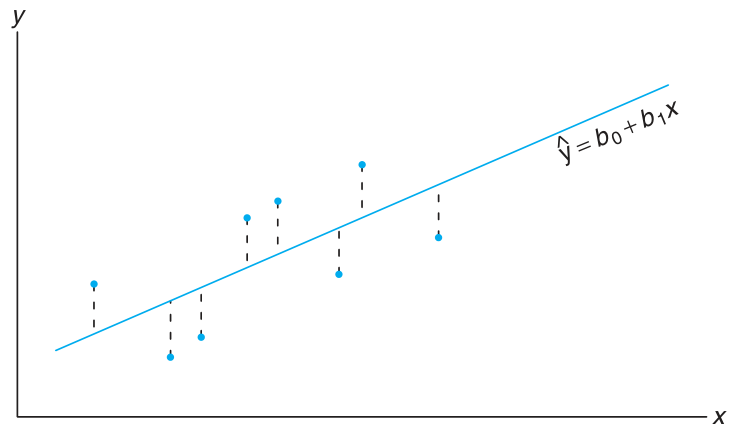
\includegraphics[width=0.7\textwidth]{leastSquares}
            \caption{Errors/residuals as vertical deviations.}
            \label{fig:leastSquares}
        \end{figure}
    \item Deming regression uses geometric distance -- better for independent errors in $x_i$ and $y_i$ 
    \item for linear regression we don't need to know $\sigma$, but for Deming we need to know the ratio of variances of $x$ and $y $ errors
\end{itemize}
\textbf{Example with Maximum Likelihood}:
\begin{itemize}
    \item recall MLE 
    \item in this case, each error $e_i$ is a realization of a normal RV $E_i$ with $\mu=0$ and variance $\sigma^2$
        \begin{itemize}
            \item this implies that each $y_i$ is also an RV with a mean of $ax_i - b$ and variance $\sigma^2$
        \end{itemize}
    \item parameters: $\theta = (a, b)$ 
    \item likelihood function: 
        \begin{gather*}
            L(e_1, \ldots, e_n; a,b) = \prod_{i=1}^{n} \frac{1}{\sqrt{2\pi} \sigma} e^{e_i^2 / 2\sigma^2} 
        .\end{gather*}
    \item maximizing this function over $(a,b)$ gives the least squares solution
\end{itemize}


\section{Properties of the Least Squares Estimators}
\textbf{Conclusion}:
\begin{itemize}
    \item if we assume $y_i=ax_i + b + e_i$
    \item $e_i$ is a realization of the normal RV $E_i$ with $\mu=0$ and variance $\sigma^2$ 
    \item $y_i$ is also a realization of RV $Y_i$ and is a function of $E_i$ 
    \item then $a$ and $b$ are realizations of RVs $A$ and $B$ 
    \item we see that $A$ and $B$ are \textbf{unbiased estimators of the true coefficients $\alpha$ and $\beta$} 
\end{itemize}

\subsection{Estimating the Error}
\begin{itemize}
    \item if $y_i = ax_i+b+e_i$ and $e_i$ is a realization of an RV $E_i$ with variance $\sigma^2$, then $\sigma^2$ reflects random variation or experimental error variation around the regression line
    \item the total squared error is 
        \begin{gather*}
            \sum_{i=1}^{n} e_i^2
        .\end{gather*}
    \item we define the statistic 
        \begin{gather*}
            S^2 = \frac{\sum_{i=1}^{n} E_i^2}{n-2}
        .\end{gather*}
    \item this is an unbiased estimator of $\sigma^2$ 
    \item if we denote the regression estimate as $\hat{y}_i = ax_i + b$ then $e_i = y_i - \hat{y}_i$
    \item we can write a realization of this as the following:
\end{itemize}
\begin{theorem}
    An unbiased estimate of $\sigma^2$ is 
    \begin{align*}
        s^2 &= \sum_{i=1}^{n} \frac{(y_i - \hat{y}_i)^2}{n-2} \\ 
            &= \frac{\sum_{i=1}^{n} (y_i - \overline{y})^2 - \alpha \sum_{i=1}^{n} (x_i-\overline{x})(y_i-\overline{y})}{n-2}
    .\end{align*}
\end{theorem}








\end{document}
